\documentclass{beamer}
%kdfj
\usetheme[secheader]{Boadilla}
\setbeamertemplate{footline} {
  %\leavevmode%
  \hbox{%
  \begin{beamercolorbox}[wd=.5\paperwidth,ht=2.25ex,dp=1ex,left]{author in head/foot}%
    \usebeamerfont{author in head/foot}\hspace*{2ex}\insertshortauthor~~(adraeger@cern.ch)
  \end{beamercolorbox}%
  \begin{beamercolorbox}[wd=.5\paperwidth,ht=2.25ex,dp=1ex,right]{date in head/foot}%
    \usebeamerfont{date in head/foot}\insertshorttitle,~
    \insertshortdate{}\hspace*{1em}
    \insertframenumber{} / \inserttotalframenumber\hspace*{2ex}
  \end{beamercolorbox}}%
  \vskip0pt%
}
\beamertemplatenavigationsymbolsempty

\usepackage[percent]{overpic}
\usepackage{tikz}
%\usetikzlibrary{positioning,fit,shapes.arrows,shapes.geometric,shapes.misc,shapes.multipart,calc,shadows}
\tikzstyle{every picture}+=[remember picture]
\usepackage{booktabs}
\usepackage{graphicx}
\usepackage{rotating}
\usepackage{wasysym}
\usepackage{marvosym}
\usepackage{amssymb}
\usepackage{xcolor}
\usepackage[normalem]{ulem}
\graphicspath{{../../logo/}{figures/}{../../graphic-common/}}

\usepackage{amsmath}
\usepackage{cancel}
\usepackage{xspace}
\usepackage{xcolor}

% editing
\newcommand{\todo}[1]{\textcolor{red}{{\textbf{TODO: }\textit{#1}}}\xspace}
\newcommand{\fixme}[1]{\textcolor{red}{{\textbf{FIXME: }\textit{#1}}}}

% helpers
\newcommand{\emptybox}[1]{\parbox[c][#1]{0pt}{}}

% boxes
\newcommand{\cfbox}[2]{{\color{#1}\fbox{\normalcolor#2}}}

% Sectioning
\newcommand{\qsec}[1]{Section~\ref{#1}}
\newcommand{\qfig}[1]{Fig.~\ref{#1}}
\newcommand{\qtab}[1]{Table~\ref{#1}}
\newcommand{\qeq}[1]{\eqref{#1}}

% Particles
\newcommand{\W}{\ensuremath{\text{W}}\xspace}
\newcommand{\Z}{\ensuremath{\text{Z}}\xspace}

% Processes
\newcommand{\ZInv}{\ensuremath{\text{Z}\rightarrow\nu\bar{\nu}}\xspace}
\newcommand{\ZInvJets}{\ensuremath{\text{Z}\rightarrow\nu\bar{\nu}\,+\,\text{jets}}\xspace}
\newcommand{\Zmumu}{\ensuremath{\text{Z}\rightarrow\mu\bar{\mu}}\xspace}
\newcommand{\Zll}{\ensuremath{\text{Z}\rightarrow\text{ll}}\xspace}
\newcommand{\Zee}{\ensuremath{\text{Z}\rightarrow\text{ee}}\xspace}
\newcommand{\ttbar}{\ensuremath{\text{t}\bar{\text{t}}}\xspace}
\newcommand{\bbbar}{\ensuremath{\text{b}\bar{\text{b}}}\xspace}
\newcommand{\ccbar}{\ensuremath{\text{c}\bar{\text{c}}}\xspace}
\newcommand{\wpj}{\ensuremath{\text{W}+\text{jets}}\xspace}
\newcommand{\photonJet}{\ensuremath{\gamma+\text{jet}}\xspace}
\newcommand{\photonJets}{\ensuremath{\gamma+\text{jets}}\xspace}
\newcommand{\ZJet}{\ensuremath{\text{Z}+\text{jet}}\xspace}
\newcommand{\ZJets}{\ensuremath{\text{Z}+\text{jets}}\xspace}
\newcommand{\photonZJet}{\ensuremath{\text{photon}/Z+\text{jet}}\xspace}
\newcommand{\muonJets}{\ensuremath{\mu+\text{jets}}\xspace}
\newcommand{\hadtau}{\ensuremath{\tau_{Had}}\xspace}
\newcommand{\wtotau}{\ensuremath{\text{W}\rightarrow\tau}\xspace}
\newcommand{\wtotautomu}{\ensuremath{\text{W}\rightarrow\tau\rightarrow\mu}\xspace}
\newcommand{\wtohadtau}{\ensuremath{\text{W}\rightarrow\tau_{Had}}\xspace}
\newcommand{\wtomu}{\ensuremath{\text{W}\rightarrow\mu}\xspace}
\newcommand{\wtolnu}{\ensuremath{\text{W}\rightarrow \text{l}\nu}\xspace}
\newcommand{\wtoe}{\ensuremath{\text{W}\rightarrow\text{e}}\xspace}
% Units
\newcommand{\tev}{\ensuremath{\;\text{Te}\kern-0.06667em\text{V}}\xspace}
\newcommand{\gev}{\ensuremath{\;\text{Ge}\kern-0.06667em\text{V}}\xspace}
\newcommand{\gevbrackets}{\ensuremath{\;[\text{Ge}\kern-0.06667em\text{V}]}\xspace}
\newcommand{\mev}{\ensuremath{\;\text{Me}\kern-0.06667em\text{V}}\xspace}
\newcommand{\kev}{\ensuremath{\;\text{ke}\kern-0.06667em\text{V}}\xspace}
\newcommand{\ev}{\ensuremath{\;\text{e}\kern-0.06667em\text{V}}\xspace}
\newcommand{\km}{\ensuremath{\;\text{km}}\xspace}
\newcommand{\m}{\ensuremath{\;\text{m}}\xspace}
\newcommand{\cm}{\ensuremath{\;\text{cm}}\xspace}
\newcommand{\mm}{\ensuremath{\;\text{mm}}\xspace}
\newcommand{\mum}{\ensuremath{\;\mu\text{m}}\xspace}
\newcommand{\hour}{\ensuremath{\;\text{h}}\xspace}
\newcommand{\second}{\ensuremath{\;\text{s}}\xspace}
\newcommand{\ns}{\ensuremath{\;\text{ns}}\xspace}
\newcommand{\kg}{\ensuremath{\;\text{kg}}\xspace}
\newcommand{\tons}{\ensuremath{\;\text{t}}\xspace}
\newcommand{\tesla}{\ensuremath{\;\text{T}}\xspace}
\newcommand{\kelvin}{\ensuremath{\;\text{K}}\xspace}
\newcommand{\nbinv}{\ensuremath{\;\text{nb}^{-1}}\xspace}
\newcommand{\pbinv}{\ensuremath{\;\text{pb}^{-1}}\xspace}
\newcommand{\fbinv}{\ensuremath{\;\text{fb}^{-1}}\xspace}
\newcommand{\pb}{\ensuremath{\;\text{pb}}\xspace}
\newcommand{\fb}{\ensuremath{\;\text{fb}}\xspace}
\newcommand{\mb}{\ensuremath{\;\text{mb}}\xspace}
\newcommand{\Hz}{\ensuremath{\;\text{Hz}}\xspace}

\newcommand{\gevnospace}{\ensuremath{\text{Ge}\kern-0.06667em\text{V}}\xspace}
\newcommand{\tevnospace}{\ensuremath{\text{Te}\kern-0.06667em\text{V}}\xspace}

% Quantities
\newcommand{\et}{\ensuremath{E_{\text{T}}}\xspace}
\newcommand{\met}{\ensuremath{\slash\mkern-12mu{E}_{\text{T}}}\xspace}
\newcommand{\metvec}{\ensuremath{\slash\mkern-12mu{\vec{E}}_{\text{T}}}\xspace}
\newcommand{\jetht}{\ensuremath{H_{\text{T}}}\xspace}
\newcommand{\mht}{\ensuremath{\slash\mkern-12mu{H}_{\text{T}}}\xspace}
\newcommand{\HT}{\ensuremath{H_{\text{T}}}\xspace}
\newcommand{\MHT}{\ensuremath{\slash\mkern-12mu{H}_{\text{T}}}\xspace}
\newcommand{\pt}{\ensuremath{p_{\text{T}}}\xspace}
\newcommand{\ptsup}[1]{\ensuremath{p^{#1}_{\text{T}}}\xspace}
\newcommand{\ptvec}{\ensuremath{\vec{p}_{\text{T}}}\xspace}
\newcommand{\ptvecsup}[1]{\ensuremath{\vec{p}^{#1}_{\text{T}}}\xspace}
\newcommand{\pti}[1]{\ensuremath{p_{\text{T},#1}}\xspace}
\newcommand{\ptivec}[1]{\ensuremath{\vec{p}_{\text{T},#1}}\xspace}
\newcommand{\ptjeti}[1]{\ensuremath{p^{\text{jet#1}}_{\text{T}}}\xspace}
\newcommand{\ptsub}[1]{\ensuremath{p_{\text{T},#1}}\xspace}
\newcommand{\ptvecsub}[1]{\ensuremath{\vec{p}_{\text{T},#1}}\xspace}
\newcommand{\ptdijet}{\ensuremath{p^{\text{dijet}}_{\text{T}}}\xspace}
\newcommand{\ptave}{\ensuremath{p^{\text{ave}}_{\text{T}}}\xspace}
\newcommand{\ptavemin}{\ensuremath{p^{\text{ave,min}}_{\text{T}}}\xspace}
\newcommand{\ptavemax}{\ensuremath{p^{\text{ave,max}}_{\text{T}}}\xspace}
\newcommand{\ptgen}{\ensuremath{p^{\text{gen}}_{\text{T}}}\xspace}
\newcommand{\ptgenave}{\ensuremath{p^{\text{gen,ave}}_{\text{T}}}\xspace}
\newcommand{\ptgenrel}{\ensuremath{p^{\text{gen,rel}}_{\text{T,3}}}\xspace}
\newcommand{\ptgeni}[1]{\ensuremath{p^{\text{gen}}_{\text{T},#1}}\xspace}
\newcommand{\pthat}{\ensuremath{\hat{p}_{\text{T}}}\xspace}
\newcommand{\pthatmin}{\ensuremath{\hat{p}^{\text{min}}_{\text{T}}}\xspace}
\newcommand{\pthatmax}{\ensuremath{\hat{p}^{\text{max}}_{\text{T}}}\xspace}
\newcommand{\pttrue}{\ensuremath{p^{\text{true}_{}}_{\text{T}}}\xspace}
\newcommand{\pttruei}[1]{\ensuremath{p^{\text{true}_{}}_{\text{T,}#1}}\xspace}
\newcommand{\ptmeas}{\ensuremath{p^{\text{meas}_{}}_{\text{T}}}\xspace}
\newcommand{\ptmeasi}[1]{\ensuremath{p^{\text{meas}_{}}_{\text{T,}#1}}\xspace}
\newcommand{\ptreco}{\ensuremath{p^{\text{reco}_{}}_{\text{T}}}\xspace}
\newcommand{\ptrel}{\ensuremath{\alpha}\xspace}
\newcommand{\ptrelmax}{\ensuremath{\alpha_{\text{max}}}\xspace}
\newcommand{\ptmin}{\ensuremath{p^{\text{min}_{}}_{\text{T}}}\xspace}
\newcommand{\ptmax}{\ensuremath{p^{\text{max}_{}}_{\text{T}}}\xspace}
\newcommand{\ptcalo}{\ensuremath{p^{\text{calo}_{}}_{\text{T}}}\xspace}
\newcommand{\ptcaloi}[1]{\ensuremath{p^{\text{calo}_{}}_{\text{T},#1}}\xspace}
\newcommand{\ptparticle}{\ensuremath{p^{\text{particle}_{}}_{\text{T}}}\xspace}
\newcommand{\ptparton}{\ensuremath{p^{\text{parton}_{}}_{\text{T}}}\xspace}
\newcommand{\ptref}{\ensuremath{p^{\text{ref}_{}}_{\text{T}}}\xspace}
\newcommand{\ppgen}{\ensuremath{p^{\text{gen}}_{||}}\xspace}
\newcommand{\ppgeni}[1]{\ensuremath{p^{\text{gen}}_{||,#1}}\xspace}
\newcommand{\pp}{\ensuremath{p_{||}}\xspace}
\newcommand{\ppi}[1]{\ensuremath{p_{||,#1}}\xspace}
\newcommand{\ppirel}[1]{\ensuremath{p^{\text{rel}}_{||,#1}}\xspace}
\newcommand{\etajeti}[1]{\ensuremath{\eta^{\text{jet#1}}}\xspace}
\newcommand{\etamin}{\ensuremath{\eta^{\text{min}}}\xspace}
\newcommand{\etamax}{\ensuremath{\eta^{\text{max}}}\xspace}
\newcommand{\fasym}{\ensuremath{f_{\text{Asym}}}\xspace}
\newcommand{\fasymdata}{\ensuremath{f^{\text{Data}}_{\text{Asym}}}\xspace}
\newcommand{\fasymmc}{\ensuremath{f^{\text{MC}}_{\text{Asym}}}\xspace}
\newcommand{\fresp}{\ensuremath{f_{\text{Resp}}}\xspace}
\newcommand{\alphat}{\ensuremath{\alpha_{\text{T}}}\xspace}
\newcommand{\resp}{\ensuremath{\mathcal{R}}\xspace}
\newcommand{\respmctruth}{\ensuremath{\mathcal{R}_{\text{MC}}}\xspace}
\newcommand{\sigmatruth}{\ensuremath{\sigma_{\text{MC}}}\xspace}
\newcommand{\asym}{\ensuremath{\mathcal{A}}\xspace}
\newcommand{\datasimratio}{\ensuremath{\rho}\xspace}
\newcommand{\NJets}{\ensuremath{N_{\text{jets}}}\xspace}
\newcommand{\BTags}{\ensuremath{B_{\text{tags}}}\xspace}
\newcommand{\Mass}[1]{\ensuremath{\text{M}_{\text{#1}}\xspace}}
\newcommand{\mass}[1]{\ensuremath{\text{m}_{\text{#1}}\xspace}}
\newcommand{\mtw}{\ensuremath{m_{T}(\text{W})\xspace}}
\newcommand{\mt}{\ensuremath{m_{T}\xspace}}

\newcommand{\deltaphi}{\ensuremath{\Delta\phi}\xspace}
\newcommand{\mindeltaphi}{\ensuremath{\Delta\phi_{N}^{min}}\xspace}
\newcommand{\dphin}{\ensuremath{\Delta \hat\phi_{\mathrm{min}}}\xspace}
\newcommand{\deltaR}{\ensuremath{\Delta R}\xspace}

% Symbols
\newcommand{\dif}[1]{\ensuremath{\text{d}#1}\xspace}
\newcommand{\e}{\,\text{e}}
\newcommand{\nup}[1]{$^{\text{\scriptsize #1}}$}
\newcommand{\dgr}{\ensuremath{\,^{\circ}}}
\newcommand{\mean}[1]{\ensuremath{\langle#1\rangle}}
\newcommand{\gqq}[1]{\ensuremath{\glqq#1\grqq}}
\newcommand{\rarr}{\ensuremath{\rightarrow}\xspace}

% Words and characters
\newcommand{\sm}{SM\xspace}
\newcommand{\diagonalsout}[1]{\ensuremath{\cancel{\text{#1}}}}
\newcommand{\genjet}{GenJet\xspace}
\newcommand{\genjets}{GenJets\xspace}
\newcommand{\calojet}{CaloJet\xspace}
\newcommand{\calojets}{CaloJets\xspace}
\newcommand{\window}[2]{\ensuremath{#1-#2\,\sigma}}
\newcommand{\windowinf}[1]{\ensuremath{#1\,\sigma - \infty}}
\newcommand{\pythia}{\textsc{Pythia}\xspace}
\newcommand{\pythiasix}{\textsc{Pythia6}\xspace}
\newcommand{\herwigpp}{\textsc{Herwig++}\xspace}
\newcommand{\herwig}{\textsc{Herwig}\xspace}
\newcommand{\madgraph}{\textsc{Madgraph}\xspace}
\newcommand{\CL}{C.\,L.\xspace}

% Jet related
\newcommand{\antikt}{anti-$k_{\text{T}}$\xspace}

% SUSY related
\newcommand{\susy}{SUSY\xspace}
\newcommand{\mssm}{MSSM\xspace}
\newcommand{\cmssm}{cMSSM\xspace}
\newcommand{\pmssm}{pMSSM\xspace}
\newcommand{\lsp}{LSP\xspace}
\newcommand{\mzero}{\ensuremath{m_{0}}\xspace}
\newcommand{\monehalf}{\ensuremath{m_{1/2}}\xspace}
\newcommand{\squark}{\ensuremath{\tilde{q}}\xspace}
\newcommand{\gluino}{\ensuremath{\tilde{g}}\xspace}
\newcommand{\msquark}{\ensuremath{m_{\tilde{q}}}\xspace}
\newcommand{\mgluino}{\ensuremath{m_{\tilde{g}}}\xspace}
\newcommand{\mneutralino}{\ensuremath{m_{\tilde{\chi}^{0}}}\xspace}
\newcommand{\tanbeta}{\ensuremath{\tan\beta}\xspace}
\newcommand{\stau}{\ensuremath{\tilde{\tau}}\xspace}
\newcommand{\neutralino}{\ensuremath{\tilde{\chi}^{0}}\xspace}

% Higgs related
\newcommand{\phitobb}{\ensuremath{\Phi\rightarrow\text{b}\bar{\text{b}}}\xspace}
\newcommand{\mhiggs}{\ensuremath{m_{\text{H}}}\xspace}
\newcommand{\mA}{\ensuremath{m_{\text{A}}}\xspace}
\newcommand{\mh}{\ensuremath{m_{\text{h}}}\xspace}
\newcommand{\mH}{\ensuremath{m_{\text{H}}}\xspace}
\newcommand{\mPhi}{\ensuremath{M_{\Phi}}\xspace}
\newcommand{\btageff}{\ensuremath{\epsilon(\text{b-tag})}\xspace}
\newcommand{\mjj}{\ensuremath{M_{12}}\xspace}
\newcommand{\xjjj}{\ensuremath{X_{123}}\xspace}
\newcommand{\mhmax}{\ensuremath{m^{\text{max}}_{h}}\xspace}


% Abbrevations
\newcommand{\etc}{etc.\ }
\newcommand{\wrt}{w.\,r.\,t.\ }
\newcommand{\cf}{cf.\ }
\newcommand{\ie}{i.\,e.\ }
\newcommand{\siehe}{s.\ }
\newcommand{\zb}{z.\,B.\ }
\newcommand{\ca}{ca.\ }
\newcommand{\eg}{e.\,g.\ }
\newcommand{\vs}{vs.\ }
\newcommand{\NB}{N.\,B.\xspace}

% Misc
\newcommand{\solidline}[1]{\textcolor{#1}{---}}
\newcommand{\dashedline}[1]{\textcolor{#1}{- -}}
\newcommand{\opencircle}[1]{\textcolor{#1}{$\circ$}}
\newcommand{\solidcircle}[1]{\textcolor{#1}{$\bullet$}}
\newcommand{\solidsquare}[1]{\textcolor{#1}{\small $\blacksquare$}}
\newcommand{\solidtriangle}[1]{\textcolor{#1}{\small $\blacktriangle$}}
\newcommand{\opensquare}[1]{\textcolor{#1}{\small $\square$}}
\newcommand{\opentriangle}[1]{\textcolor{#1}{\small $\triangle$}}
\newcommand{\opendiamond}[1]{\textcolor{#1}{\small $\diamond$}}
\newcommand{\greencheck}{\textcolor{beamerGreen}{\ensuremath{\checkmark}}\xspace}
\newcommand{\bibbullet}{\includegraphics[width=1em]{../../graphic-common/eyeCandy/freehand-book.png}}

% Colours
\definecolor{beamerGreen}{rgb}{0,0.6,0}
\definecolor{darkGreen}{rgb}{0,0.6,0}
\definecolor{beamerYellow}{rgb}{1.,0.745,0}
\definecolor{gray}{rgb}{0.4,0.4,0.4}
\definecolor{darkgreen}{RGB}{000,100,000}
\definecolor{kGreen2}{RGB}{000,153,000}
\definecolor{theme_blue}{RGB}{051,051,178}
\definecolor{theme_blue_light}{HTML}{ADADE0}

\newcommand{\blue}[1]{\textcolor{blue}{#1}}
\newcommand{\themeblue}[1]{\textcolor{theme_blue}{#1}}
\newcommand{\red}[1]{\textcolor{red}{#1}}
\newcommand{\orange}[1]{\textcolor{orange}{#1}}
\newcommand{\green}[1]{\textcolor{green}{#1}}
\newcommand{\yellow}[1]{\textcolor{yellow}{#1}}
\newcommand{\white}[1]{\textcolor{white}{#1}}
\newcommand{\grey}[1]{\textcolor{gray}{#1}}
\newcommand{\link}[2]{\href{#1}{\textcolor{theme_blue}{\underline{#2}}}}

% Libre-Office colours
\definecolor{oochart2}{HTML}{FF420E}  % orange
\definecolor{oochart7}{HTML}{314004}  % dark green
\definecolor{oochart11}{RGB}{197,001,012} % dark red
\definecolor{oochart12}{RGB}{001,132,209} % light blue


% ROOT colors
\definecolor{kBlack}{HTML}{000000}
\definecolor{kRed}{HTML}{FF0000}
\definecolor{kRedUp2}{HTML}{6B0C0C}
\definecolor{kYellow}{HTML}{FEFE12}
\definecolor{kBlue}{HTML}{0000FF}
\definecolor{kOrange}{HTML}{FFCC00}
\definecolor{kGreen}{HTML}{59D454}
\definecolor{kGreenUp2}{HTML}{009900}
\definecolor{kMagenta}{HTML}{FF00FF}
\definecolor{kCyan}{HTML}{00FFFF}

% Colored symbols
\newcommand{\mysquare}[1][black]{\scriptsize\textcolor{#1}{\ensuremath\blacksquare}}
\newcommand{\mycirc}[1][black]{\scriptsize\textcolor{#1}{\ensuremath\bullet}}
\newcommand{\mylozenge}[1][black]{\small\textcolor{#1}{\ensuremath\blacklozenge}}
\newcommand{\mytriangle}[1][black]{\small\textcolor{#1}{\ensuremath\blacktriangle}}
\newcommand{\mydtriangle}[1][black]{\small\textcolor{#1}{\ensuremath\blacktriangledown}}
\newcommand{\mystar}[1][black]{\Large\textcolor{#1}{\ensuremath\star}} %% or \bigstar

\newcommand{\lib}[1]{\tiny #1}

% Title etc
\vskip2cm
\title[RA2/b Meeting]{Classical Lost-Lepton Background}
\subtitle{Tag \& Probe Efficiencies (Update) \\ Isolated Tracks Implementation in Method}
\author[Arne-Rasmus~Dr\"ager]{
  Arne-Rasmus~Dr\"ager(Uni Hamburg)
}
\date[June 09, 2015]{June 09, 2015
  \vskip1cm
  \begin{center}
    
\includegraphics[height=1.5cm]{Universitaet-Hamburg-Logo.jpg}
    \hskip8cm
    
\includegraphics[height=1.5cm]{CMSlogo.jpeg}
  \end{center}
}

% pdflatex packages
\hypersetup{bookmarks=true}
\hypersetup{unicode=false}
\hypersetup{pdftitle={Lost-Lepton}}
\hypersetup{pdfauthor={Arne-Rasmus~Dr\"ager}}


\begin{document}
% ==================================================
% --------------------------------------------------
\begin{frame}
  \titlepage
\end{frame}

\section{Classical Lost-Lepton Method}
\begin{frame}
 \begin{block}{}
 \centering
 \Large Classical Lost-Lepton Method
 \end{block}
\end{frame}
\subsection{Concept}
\begin{frame}
 \begin{center}
\begin{tikzpicture}
    \node[anchor=south west,inner sep=0] (image) at (0,0) {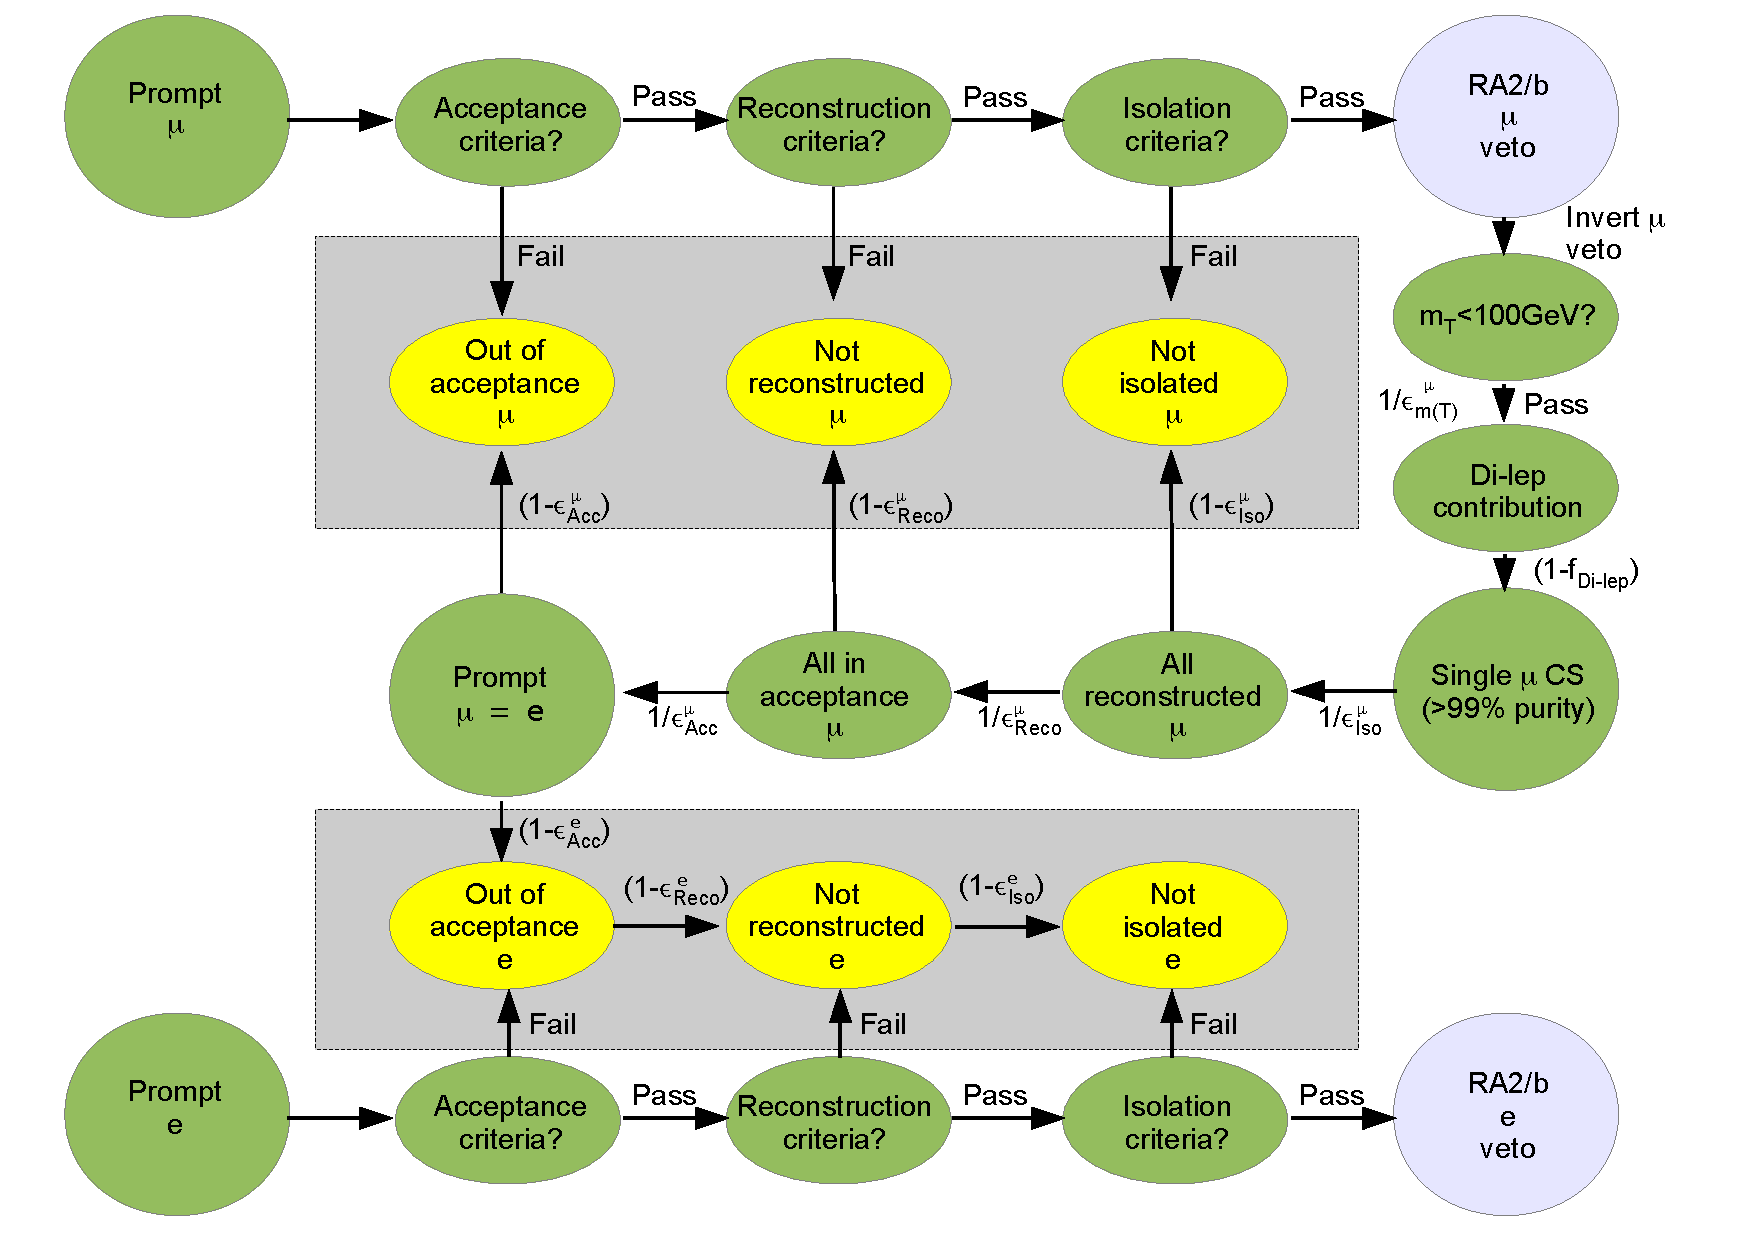
\includegraphics[width=0.75\textwidth]{figures/Sketches/LostLeptonSketch_mu_pred_full.pdf}};
    \begin{scope}[x={(image.south east)},y={(image.north west)}]
%         \draw[red,ultra thick,rounded corners] (0.62,0.65) rectangle (0.78,0.75);
%         \draw[red,ultra thick,rounded corners] (0.60,0.01) rectangle (0.75,0.99); % coordinates unten links(x,y) oben rechts(x,y)
%             \draw[blue,ultra thick,rounded corners] (0.40,0.01) rectangle (0.55,0.99); % coordinates unten links(x,y) oben rechts(x,y)
    \end{scope}
\end{tikzpicture}
\subsection{Closure}
 \end{center}
\end{frame}
\begin{frame}
\frametitle{Full closure-test of the classical lost-lepton method}
  \begin{columns}
    \begin{column}{0.5\textwidth}
     \centering
      \begin{overpic}[width=0.70\textwidth]{figures/lost-lepton_classic/Closure/Baseline/Closure__HT__MCEx_vs_MuPrMTWDiLep+ElecPrMTWDiLep__Baseline.pdf}%\put(100,60){\rotatebox{-90}{\scriptsize Old Parametrization Variables}}
     \end{overpic}
      \begin{overpic}[width=0.70\textwidth]{figures/lost-lepton_classic/Closure/Baseline/Closure__NJets__MCEx_vs_MuPrMTWDiLep+ElecPrMTWDiLep__Baseline.pdf}
     \end{overpic}
    \end{column}
    \begin{column}{0.5\textwidth}
      \centering
      \begin{overpic}[width=0.70\textwidth]{figures/lost-lepton_classic/Closure/Baseline/Closure__MHT__MCEx_vs_MuPrMTWDiLep+ElecPrMTWDiLep__Baseline.pdf} %\put(100,60){\rotatebox{-90}{\scriptsize New Parametrization Variables}}    
      \end{overpic}
      \centering
      \begin{overpic}[width=0.70\textwidth]{figures/lost-lepton_classic/Closure/Baseline/Closure__BTags__MCEx_vs_MuPrMTWDiLep+ElecPrMTWDiLep__Baseline.pdf}     \end{overpic}
    \end{column}
  \end{columns}
\end{frame}

\begin{frame}
%  \frametitle{Closure test in each search bin}
 \begin{center}
  \begin{overpic}[width=0.55\textwidth]{figures/lost-lepton_classic/Closure/Baseline/Closure__Bin__MCEx_vs_MuPrMTWDiLep+ElecPrMTWDiLep__Baseline.pdf}      \put(18,36.2){\color{red}\line(1,0){75}}
      \end{overpic}
 \end{center}
\begin{itemize}
 \item Overall good closure observed in most search bins. Still room for improvement!
 \item In extrem phase-space low statistics of control-sample!
\end{itemize}


\end{frame}
\begin{frame}
 \frametitle{Lost single $\mu/e$ Control-Sample Issue}
  \begin{columns}
    \begin{column}{0.5\textwidth}
     \begin{itemize}
  \item Many extrem phase-space bins suffer from no expected single $\mu/e$ control-sample. Very true for most sensitive search bins.
   \item Approach to solve this for classical lost-lepton method:
  \end{itemize}
  
    \end{column}
  \begin{column}{0.5\textwidth}
  
  \begin{overpic}[width=1\textwidth]{figures/lost-lepton_classic/Simon/Mean_Prediction.pdf} %\put(100,60){\rotatebox{-90}{\scriptsize New Parametrization Variables}}    
      \end{overpic}
    \end{column}
  \end{columns}
  \begin{itemize}
   \item 0 $\mu/e$ control-sample get a predictino of 0 with an upper uncertainty of 1.82 * avarge weight from MC in that particular bin
   \item Even availabe MC statistics are not sufficient in some of thous bins. Combine avarge weight in bins with similar prediction (integrate over \BTags!?)
 \end{itemize}

\end{frame}



%%%%%%%%%%%%%%%%%%%%%%%%%%%%%%%%%%%%%%%%%%%
\section{Extrapolation Lost-Lepton Method}
\begin{frame}
 \begin{block}{}
 \centering
 \Large \MHT Extrapolation Method\\  \small Jack \& Owen
 \end{block}
\end{frame}

\begin{frame}
 \frametitle{The Idea}
 \begin{itemize}
  \item Use MC to build a \MHT PDF to take our data-driven BG estimation in the lowest \MHT bins (high CS statistics) extrapolate to higher \MHT bins (low CS statistics)
 \end{itemize}
  \begin{columns}
  \begin{column}{0.45\textwidth}
   \begin{itemize}
    \item Neutrino spectrum depends on:
    \begin{enumerate}
     \item W angular decay distribution (known to high precision)
     \item t/W-\pt spectrum, ISR, etc (tricky)
    \end{enumerate}
    \end{itemize}
    \begin{enumerate}
     \item can be taken from MC 
     \item Measure from Data
    \end{enumerate}
  \end{column}
  \begin{column}{0.55\textwidth}
   \begin{tikzpicture}
    \node[anchor=south west,inner sep=0] (image) at (0,0) {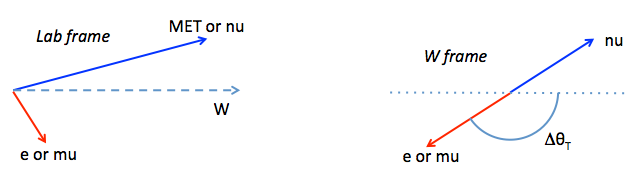
\includegraphics[width=1.\textwidth]{figures/Sketches/MHTExtrapolation.png}};
    \begin{scope}[x={(image.south east)},y={(image.north west)}]
   \end{scope}
   \end{tikzpicture}
   \begin{tikzpicture}
    \node[anchor=south west,inner sep=0] (image) at (0,0) {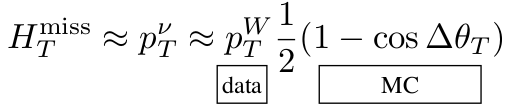
\includegraphics[width=1.\textwidth]{figures/Sketches/Extrapolation_MHT_Equation.png}};
    \begin{scope}[x={(image.south east)},y={(image.north west)}]
   \end{scope}
   \end{tikzpicture}
  \end{column}
 \end{columns}
\end{frame}
\begin{frame}
 \frametitle{Concept of the Method}
 \begin{itemize}
  \item Create \MHT PDFs using all events in the SL CS with $\pt(\text{W})>200\gev$
  \item For each SL data event we do:
 \end{itemize}
 \begin{overpic}[width=\textwidth]{figures/Sketches/Extrapolation_FullProcedure.png}
   \put(25,40){\textcolor{white}{\large \bf MC}}
 \end{overpic}
 \begin{itemize}
  \item Integrating over all events $\rightarrow$ full \MHT shape for a given \HT-\NJets bin
  \item Apply classical lost-lepton method in lowest \MHT bin in each \HT-\MHT-\NJets-\BTags bin to obtain normalization
 \end{itemize}


\end{frame}

\begin{frame}
 \frametitle{Extrapolation in \MHT from calssical estimation method}
 \begin{itemize}
  \item Extrapolation gives low-to-high \MHT ratios
 \end{itemize}
 \begin{columns}
  \begin{column}{0.55\textwidth}
   \begin{itemize}
    \item Within a given \NJets \& \BTags bin Normalizations:
    \begin{itemize}
     \item Box 1+2 for Box 4
     \item Box 3 for Box 5
     \item Box 2+3 for Box 6
    \end{itemize}
    \item Extrapolation ratios binned \NJets \& \HT, not \BTags
   \end{itemize}
 \begin{overpic}[width=\textwidth]{figures/Extrapolation/Ratios.png}
   \put(25,40){\textcolor{white}{\large \bf MC}}
 \end{overpic}
  \end{column}
  \begin{column}{0.45\textwidth}
   \begin{overpic}[width=\textwidth]{figures/Sketches/ExtrapolationFactorBoxes.png}
   \put(25,40){\textcolor{white}{\large \bf MC}}
   \end{overpic}
  \end{column}
  \end{columns}

\end{frame}

\begin{frame}
\frametitle{Comparison Closure: $\BTags\ge3, 4\ge\NJets\ge6$ }
\begin{columns}
\centering
           \begin{column}{0.50\textwidth}
     \begin{tikzpicture}
    \node[anchor=south west,inner sep=0] (image) at (0,0) {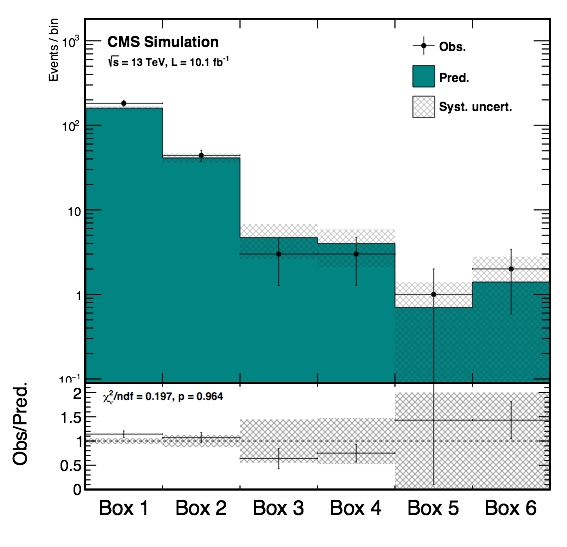
\includegraphics[width=.8\textwidth]{figures/Extrapolation/Closure_Classical_b3NJets4-6.png}};
    \begin{scope}[x={(image.south east)},y={(image.north west)}]
   
%     \draw[red,ultra thick,rounded corners] (0.62,0.65) rectangle (0.78,0.75);
       % \draw[red,ultra thick,rounded corners] (0.60,0.01) rectangle (0.75,0.99); % coordinates unten links(x,y) oben rechts(x,y)
          %  \draw[blue,ultra thick,rounded corners] (0.40,0.01) rectangle (0.55,0.99); % coordinates unten links(x,y) oben rechts(x,y)
    \end{scope}
\end{tikzpicture}
   \end{column}
   
           \begin{column}{0.50\textwidth}
           \centering
     \begin{tikzpicture}
    \node[anchor=south west,inner sep=0] (image) at (0,0) {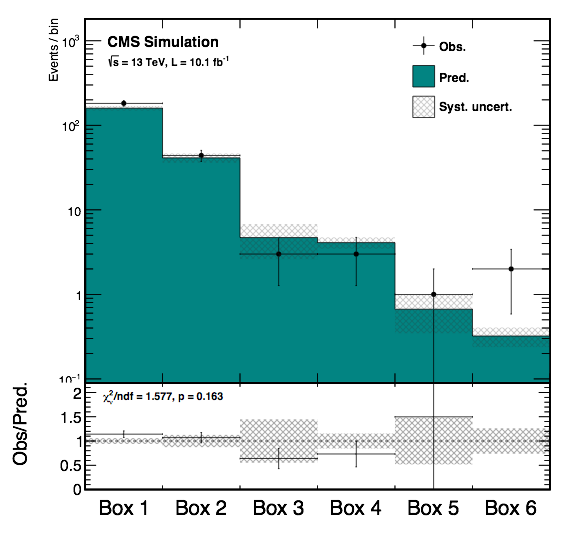
\includegraphics[width=.8\textwidth]{figures/Extrapolation/Closure_Extrapolation_b3NJets4-6.png}};
    \begin{scope}[x={(image.south east)},y={(image.north west)}]
     \put(77.,128){\color{red}\line(0,-1){113}}
%         \draw[red,ultra thick,rounded corners] (0.62,0.65) rectangle (0.78,0.75);
       % \draw[red,ultra thick,rounded corners] (0.60,0.01) rectangle (0.75,0.99); % coordinates unten links(x,y) oben rechts(x,y)
          %  \draw[blue,ultra thick,rounded corners] (0.40,0.01) rectangle (0.55,0.99); % coordinates unten links(x,y) oben rechts(x,y)
    \end{scope}
\end{tikzpicture}
   \end{column}
    \end{columns}
\begin{columns}
 \begin{column}{0.60\textwidth}
  \begin{tikzpicture}
    \node[anchor=south west,inner sep=0] (image) at (0,0) {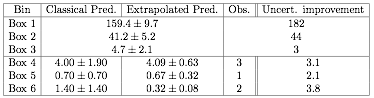
\includegraphics[width=1.\textwidth]{figures/Extrapolation/Table_b3NJets4-6.png}};
    \begin{scope}[x={(image.south east)},y={(image.north west)}]
%      \put(77.,128){\color{red}\line(0,-1){113}}
%         \draw[red,ultra thick,rounded corners] (0.62,0.65) rectangle (0.78,0.75);
       % \draw[red,ultra thick,rounded corners] (0.60,0.01) rectangle (0.75,0.99); % coordinates unten links(x,y) oben rechts(x,y)
          %  \draw[blue,ultra thick,rounded corners] (0.40,0.01) rectangle (0.55,0.99); % coordinates unten links(x,y) oben rechts(x,y)
    \end{scope}
\end{tikzpicture}
 \end{column}
 \begin{column}{0.40\textwidth}
  \begin{itemize}
  \small
   \item Shift in prediction of Boxes 4-5
   \item Box 6 underpredicted with extrapolation
   \item Reduction of uncertainty factor 2-4 $\rightarrow$ factor 4-16 gain in stats. 
  \end{itemize}

 \end{column}
\end{columns}

\end{frame}


\begin{frame}
\frametitle{Comparison Closure: $\BTags\ge3, 7\ge\NJets\ge8$ }
\begin{columns}
\centering
           \begin{column}{0.50\textwidth}
     \begin{tikzpicture}
    \node[anchor=south west,inner sep=0] (image) at (0,0) {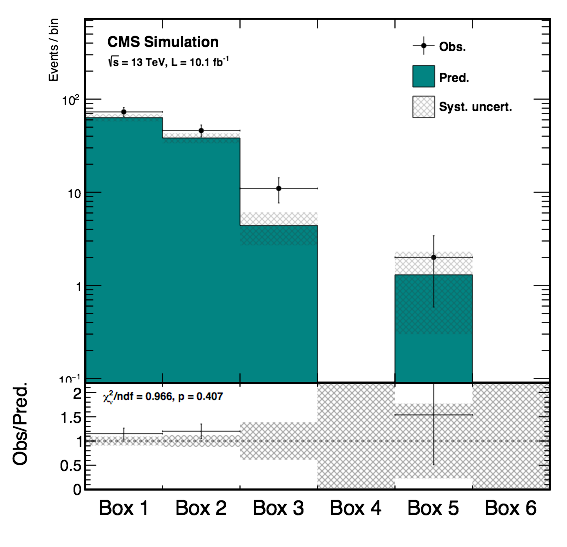
\includegraphics[width=.8\textwidth]{figures/Extrapolation/Closure_Classical_b3NJets7-8.png}};
    \begin{scope}[x={(image.south east)},y={(image.north west)}]
   
%     \draw[red,ultra thick,rounded corners] (0.62,0.65) rectangle (0.78,0.75);
       % \draw[red,ultra thick,rounded corners] (0.60,0.01) rectangle (0.75,0.99); % coordinates unten links(x,y) oben rechts(x,y)
          %  \draw[blue,ultra thick,rounded corners] (0.40,0.01) rectangle (0.55,0.99); % coordinates unten links(x,y) oben rechts(x,y)
    \end{scope}
\end{tikzpicture}
   \end{column}
   
           \begin{column}{0.50\textwidth}
           \centering
     \begin{tikzpicture}
    \node[anchor=south west,inner sep=0] (image) at (0,0) {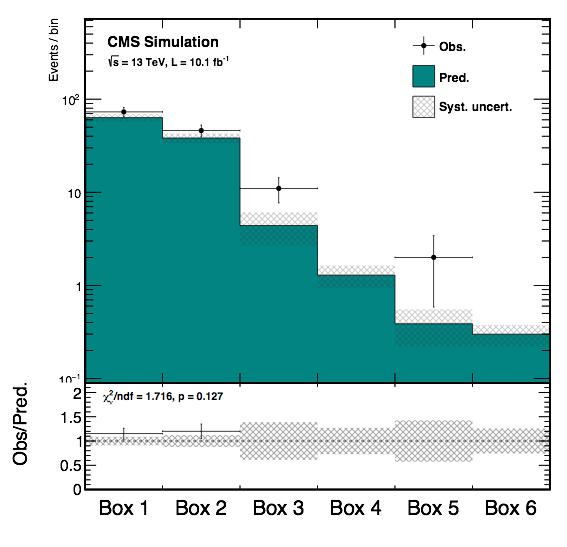
\includegraphics[width=.8\textwidth]{figures/Extrapolation/Closure_Extrapolation_b3NJets7-8.png}};
    \begin{scope}[x={(image.south east)},y={(image.north west)}]
     \put(77.,128){\color{red}\line(0,-1){113}}
%         \draw[red,ultra thick,rounded corners] (0.62,0.65) rectangle (0.78,0.75);
       % \draw[red,ultra thick,rounded corners] (0.60,0.01) rectangle (0.75,0.99); % coordinates unten links(x,y) oben rechts(x,y)
          %  \draw[blue,ultra thick,rounded corners] (0.40,0.01) rectangle (0.55,0.99); % coordinates unten links(x,y) oben rechts(x,y)
    \end{scope}
\end{tikzpicture}
   \end{column}
    \end{columns}
\begin{columns}
 \begin{column}{0.60\textwidth}
  \begin{tikzpicture}
    \node[anchor=south west,inner sep=0] (image) at (0,0) {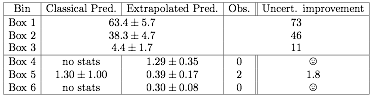
\includegraphics[width=1.\textwidth]{figures/Extrapolation/Table_b3NJets7-8.png}};
    \begin{scope}[x={(image.south east)},y={(image.north west)}]
%      \put(77.,128){\color{red}\line(0,-1){113}}
%         \draw[red,ultra thick,rounded corners] (0.62,0.65) rectangle (0.78,0.75);
       % \draw[red,ultra thick,rounded corners] (0.60,0.01) rectangle (0.75,0.99); % coordinates unten links(x,y) oben rechts(x,y)
          %  \draw[blue,ultra thick,rounded corners] (0.40,0.01) rectangle (0.55,0.99); % coordinates unten links(x,y) oben rechts(x,y)
    \end{scope}
\end{tikzpicture}
 \end{column}
 \begin{column}{0.40\textwidth}
  \begin{itemize}
  \small
   \item Achieve an effective control-sample in previously empty 2 bins!
  \end{itemize}

 \end{column}
\end{columns}

\end{frame}

\begin{frame}
\frametitle{Comparison Closure: $\BTags\ge3, 9\ge\NJets$ }
\begin{columns}
\centering
           \begin{column}{0.50\textwidth}
     \begin{tikzpicture}
    \node[anchor=south west,inner sep=0] (image) at (0,0) {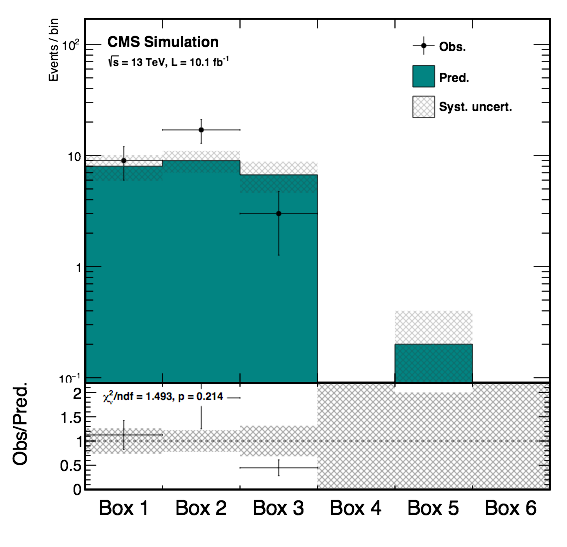
\includegraphics[width=.8\textwidth]{figures/Extrapolation/Closure_Classical_b3NJets9+.png}};
    \begin{scope}[x={(image.south east)},y={(image.north west)}]
   
%     \draw[red,ultra thick,rounded corners] (0.62,0.65) rectangle (0.78,0.75);
       % \draw[red,ultra thick,rounded corners] (0.60,0.01) rectangle (0.75,0.99); % coordinates unten links(x,y) oben rechts(x,y)
          %  \draw[blue,ultra thick,rounded corners] (0.40,0.01) rectangle (0.55,0.99); % coordinates unten links(x,y) oben rechts(x,y)
    \end{scope}
\end{tikzpicture}
   \end{column}
   
           \begin{column}{0.50\textwidth}
           \centering
     \begin{tikzpicture}
    \node[anchor=south west,inner sep=0] (image) at (0,0) {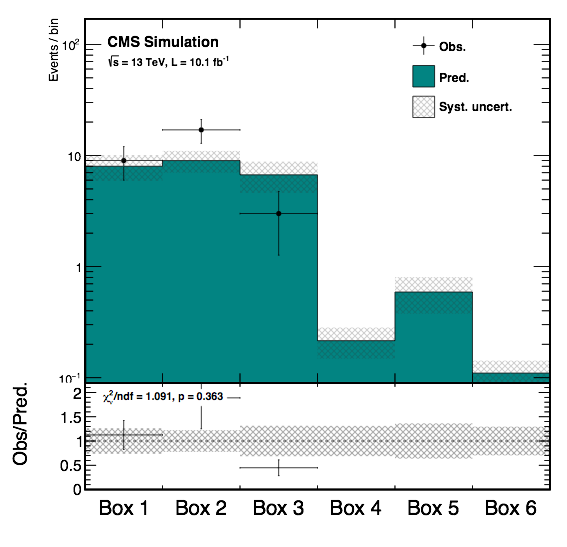
\includegraphics[width=.8\textwidth]{figures/Extrapolation/Closure_Extrapolation_b3NJets9+.png}};
    \begin{scope}[x={(image.south east)},y={(image.north west)}]
     \put(77.,128){\color{red}\line(0,-1){113}}
%         \draw[red,ultra thick,rounded corners] (0.62,0.65) rectangle (0.78,0.75);
       % \draw[red,ultra thick,rounded corners] (0.60,0.01) rectangle (0.75,0.99); % coordinates unten links(x,y) oben rechts(x,y)
          %  \draw[blue,ultra thick,rounded corners] (0.40,0.01) rectangle (0.55,0.99); % coordinates unten links(x,y) oben rechts(x,y)
    \end{scope}
\end{tikzpicture}
   \end{column}
    \end{columns}
\begin{columns}
 \begin{column}{0.60\textwidth}
  \begin{tikzpicture}
    \node[anchor=south west,inner sep=0] (image) at (0,0) {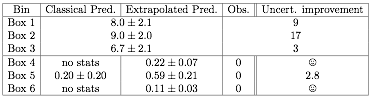
\includegraphics[width=1.\textwidth]{figures/Extrapolation/Table_b3NJets9+.png}};
    \begin{scope}[x={(image.south east)},y={(image.north west)}]
%      \put(77.,128){\color{red}\line(0,-1){113}}
%         \draw[red,ultra thick,rounded corners] (0.62,0.65) rectangle (0.78,0.75);
       % \draw[red,ultra thick,rounded corners] (0.60,0.01) rectangle (0.75,0.99); % coordinates unten links(x,y) oben rechts(x,y)
          %  \draw[blue,ultra thick,rounded corners] (0.40,0.01) rectangle (0.55,0.99); % coordinates unten links(x,y) oben rechts(x,y)
    \end{scope}
\end{tikzpicture}
 \end{column}
 \begin{column}{0.40\textwidth}
  \begin{itemize}
  \small
   \item Even at $\BTags\ge3, 9\ge\NJets, \HT>1200 \gev \& 200<\MHT<500$ have control-sample now!
  \end{itemize}

 \end{column}
\end{columns}

\end{frame}

%%%%%%%%%%%%%%%%%%%%%%%%%%%%%%%%%%%%%%%%%%%

\section{Had-Tau Method}

\begin{frame}
 \begin{block}{}
 \centering
 \Large The $\tau_{Had}$ Background
 \end{block}
\end{frame}

\subsection{Concept}
\begin{frame}
 \frametitle{Basic Idea of the $\tau_{Had}$ Estimation Method}
 
    \begin{columns}
        \begin{column}{0.60\textwidth}
        \begin{itemize}
         \item Start with single $\mu$ control-sample
         \item Replace muon $\pt$ by tau response template from MC
         \item Recalculate \HT, \MHT, \NJets \& \met
         \item Also \BTags are recomputed using mistag rate of \hadtau jets
         \item Corections:
         \begin{itemize}
          \item $\mu$ acceptance [\HT,\MHT,\NJets]
          \item $\mu$ trigger, reco/ID, iso, efficiencies [\pt, activity]
          \item $\mu$ from $\tau$ decays [$\mu$ \pt, HT, MHT, \NJets]
          \item $\frac{BR(\wtohadtau)}{BR(\wtomu)}=0.64$
         \end{itemize}

        \end{itemize}
        Note: Isotrack veto not taken into account yet, need to correct predictino for isotrack efficiency.
        

        
    
   \end{column}
           \begin{column}{0.40\textwidth}
     \begin{tikzpicture}
    \node[anchor=south west,inner sep=0] (image) at (0,0) {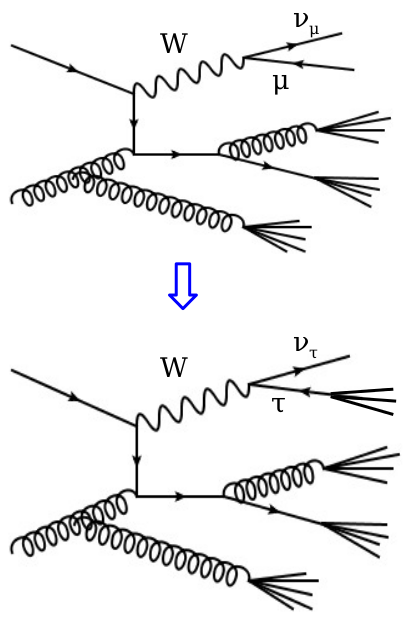
\includegraphics[width=1.\textwidth]{figures/Sketches/TauMethodSketchFenyman.png}};
    \begin{scope}[x={(image.south east)},y={(image.north west)}]
%         \draw[red,ultra thick,rounded corners] (0.62,0.65) rectangle (0.78,0.75);
       % \draw[red,ultra thick,rounded corners] (0.60,0.01) rectangle (0.75,0.99); % coordinates unten links(x,y) oben rechts(x,y)
          %  \draw[blue,ultra thick,rounded corners] (0.40,0.01) rectangle (0.55,0.99); % coordinates unten links(x,y) oben rechts(x,y)
    \end{scope}
\end{tikzpicture}
   \end{column}
    \end{columns}
\end{frame}

\subsection{Status}
\begin{frame}
 \frametitle{Closure Test as of May 17th}
 \begin{columns}
  \begin{column}{0.33\textwidth}
  \begin{itemize}
   \item Some increasing non-closure were visible for \HT, \MHT \& \NJets
   \item Conducted major investigation of source
  \end{itemize}

   \begin{tikzpicture}
    \node[anchor=south west,inner sep=0] (image) at (0,0) {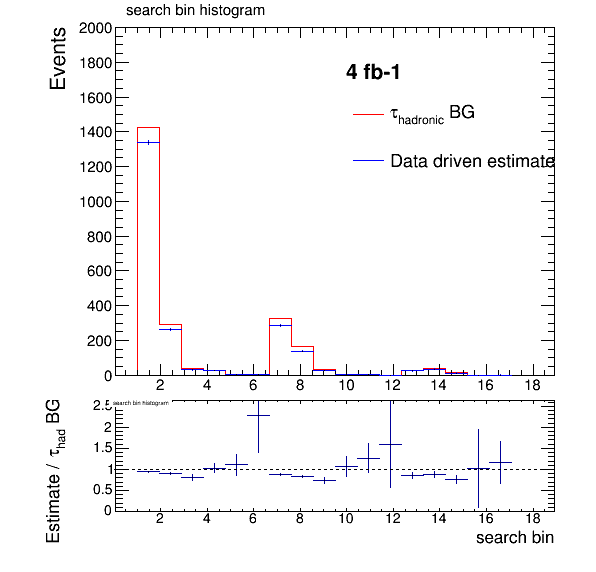
\includegraphics[width=1.\textwidth]{figures/HadTau/FromKen/Bins_FullClosure.png}};
    \begin{scope}[x={(image.south east)},y={(image.north west)}]
    \end{scope}
   \end{tikzpicture}
  \end{column}
  \begin{column}{0.33\textwidth}
   \begin{tikzpicture}
    \node[anchor=south west,inner sep=0] (image) at (0,0) {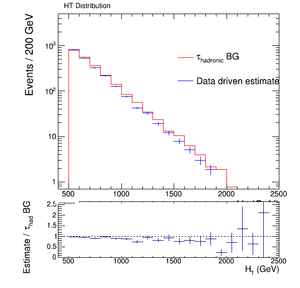
\includegraphics[width=1.\textwidth]{figures/HadTau/FromKen/HT_FullClosure.png}};
    \begin{scope}[x={(image.south east)},y={(image.north west)}]
    \end{scope}
   \end{tikzpicture}
   \begin{tikzpicture}
    \node[anchor=south west,inner sep=0] (image) at (0,0) {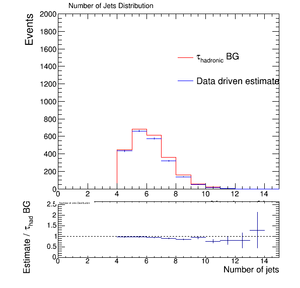
\includegraphics[width=1.\textwidth]{figures/HadTau/FromKen/NJets_FullClosure.png}};
    \begin{scope}[x={(image.south east)},y={(image.north west)}]
    \end{scope}
   \end{tikzpicture}
  \end{column}
  \begin{column}{0.33\textwidth}
   \begin{tikzpicture}
    \node[anchor=south west,inner sep=0] (image) at (0,0) {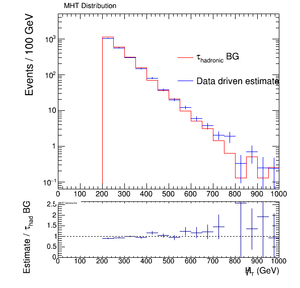
\includegraphics[width=1.\textwidth]{figures/HadTau/FromKen/MHT_FullClosure.png}};
    \begin{scope}[x={(image.south east)},y={(image.north west)}]
    \end{scope}
   \end{tikzpicture}
   \begin{tikzpicture}
    \node[anchor=south west,inner sep=0] (image) at (0,0) {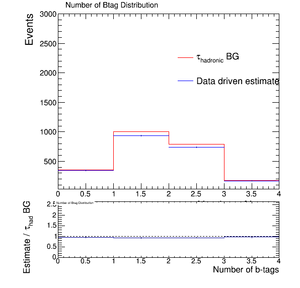
\includegraphics[width=1.\textwidth]{figures/HadTau/FromKen/BTags_FullClosure.png}};
    \begin{scope}[x={(image.south east)},y={(image.north west)}]
    \end{scope}
   \end{tikzpicture}
  \end{column}
 \end{columns}

\end{frame}
\begin{frame}
 \frametitle{Investigation of residual non-closure}
 \begin{itemize}
  \item Take out the $\mu$ corrections:
  \begin{itemize}
   \item $\mu$ acceptance [\HT,\MHT,\NJets]
   \item $\mu$ trigger, reco/ID, iso, efficiencies [\pt, activity]
   \item $\mu$ from $\tau$ decays [$\mu$ \pt, HT, MHT, \NJets]
  \end{itemize}
  \item Check consistency of:
  \item \uline{Expectation} from MC truth:
  \begin{itemize}
   \item Consider \hadtau background events wih at least one $\tau$ within $\mu$ acceptance
  \end{itemize}
  \item \uline{Data-Driven Prediction:}
  \begin{itemize}
   \item Start with gen $\mu$ directly from W decay within accpetance
   \item No $\mu$ corrections
  \end{itemize}
 \end{itemize}
 \begin{block}{}
 \centering
 \Large Check $\mu\rightarrow\hadtau$ response for consistency
 \end{block}
\end{frame}

\begin{frame}
 \frametitle{Simplified Closure}
 \begin{columns}
  \begin{column}{0.33\textwidth}
  \begin{itemize}
   \item Applied cuts:
   \begin{itemize}
    \item $\HT>500\gev$
    \item $\MHT>200\gev$
    \item $\NJets\ge4$
    \item No $\Delta\phi$ cuts
   \end{itemize}
   \item Still 7\% underprediction, but trend vs search variables improved
  \end{itemize}
  \end{column}
  \begin{column}{0.33\textwidth}
   \begin{tikzpicture}
    \node[anchor=south west,inner sep=0] (image) at (0,0) {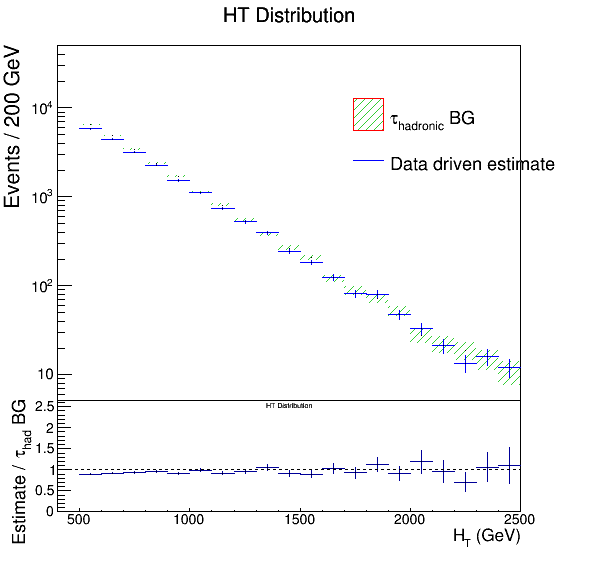
\includegraphics[width=1.\textwidth]{figures/HadTau/FromKen/HT_SimplifiedClosure1.png}};
    \begin{scope}[x={(image.south east)},y={(image.north west)}]
    \end{scope}
   \end{tikzpicture}
   \begin{tikzpicture}
    \node[anchor=south west,inner sep=0] (image) at (0,0) {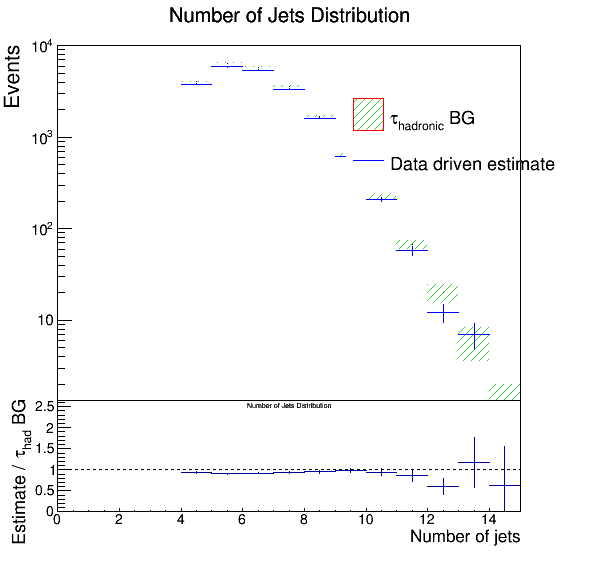
\includegraphics[width=1.\textwidth]{figures/HadTau/FromKen/NJets_SimplifiedClosure1.png}};
    \begin{scope}[x={(image.south east)},y={(image.north west)}]
    \end{scope}
   \end{tikzpicture}
  \end{column}
  \begin{column}{0.33\textwidth}
   \begin{tikzpicture}
    \node[anchor=south west,inner sep=0] (image) at (0,0) {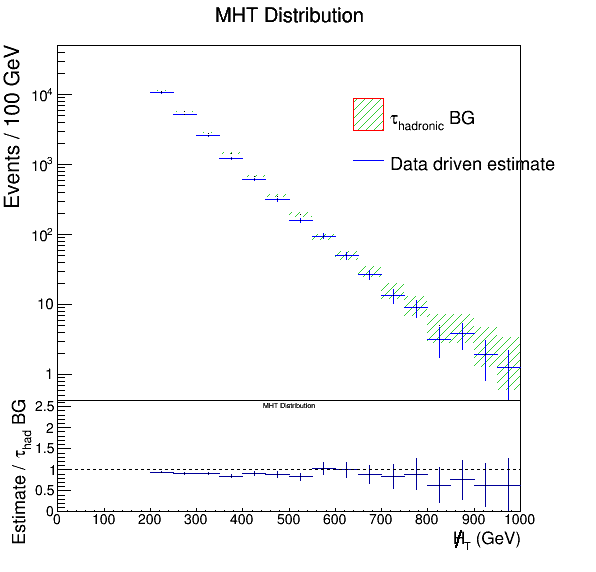
\includegraphics[width=1.\textwidth]{figures/HadTau/FromKen/MHT_SimplifiedClosure1.png}};
    \begin{scope}[x={(image.south east)},y={(image.north west)}]
    \end{scope}
   \end{tikzpicture}
   \begin{tikzpicture}
    \node[anchor=south west,inner sep=0] (image) at (0,0) {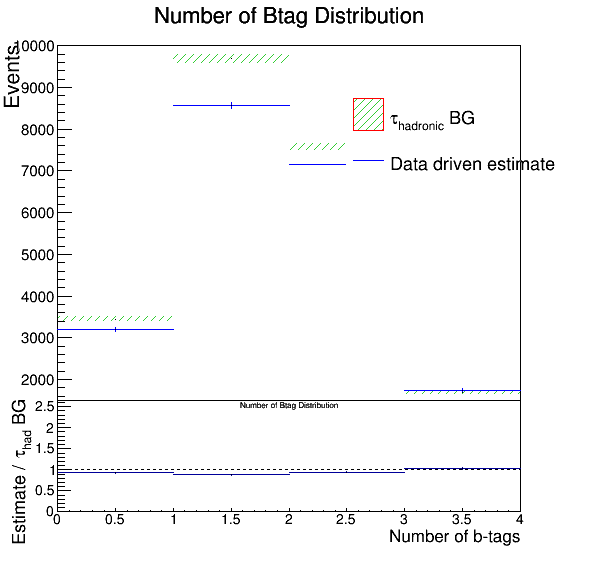
\includegraphics[width=1.\textwidth]{figures/HadTau/FromKen/BTags_SimplifiedClosure1.png}};
    \begin{scope}[x={(image.south east)},y={(image.north west)}]
    \end{scope}
   \end{tikzpicture}
  \end{column}
 \end{columns}
\end{frame}

\begin{frame}
 \frametitle{Angular Variables Closure Test}
 \begin{columns}
  \begin{column}{0.33\textwidth}
  \begin{itemize}
   \item MinDeltaPhiN is least well modeled by the method
   \item Move to simple deltaphi cuts?
  \end{itemize}
  \end{column}
  \begin{column}{0.33\textwidth}
   \begin{tikzpicture}
    \node[anchor=south west,inner sep=0] (image) at (0,0) {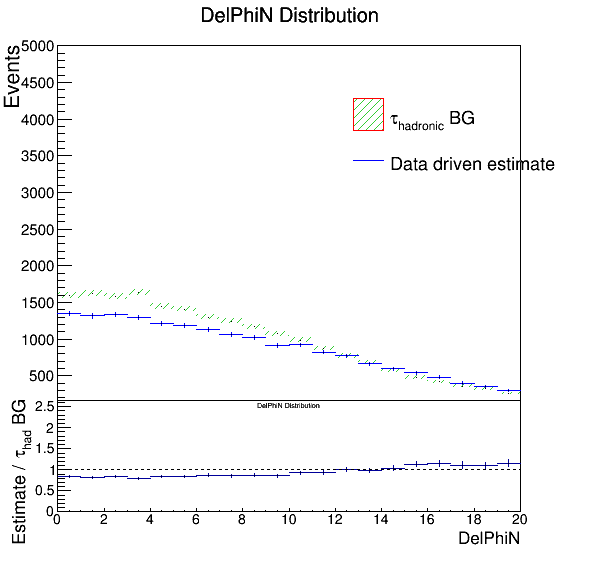
\includegraphics[width=1.\textwidth]{figures/HadTau/FromKen/MinDeltaPhiN_SimplifiedClosure1.png}};
    \begin{scope}[x={(image.south east)},y={(image.north west)}]
    \end{scope}
   \end{tikzpicture}
   \begin{tikzpicture}
    \node[anchor=south west,inner sep=0] (image) at (0,0) {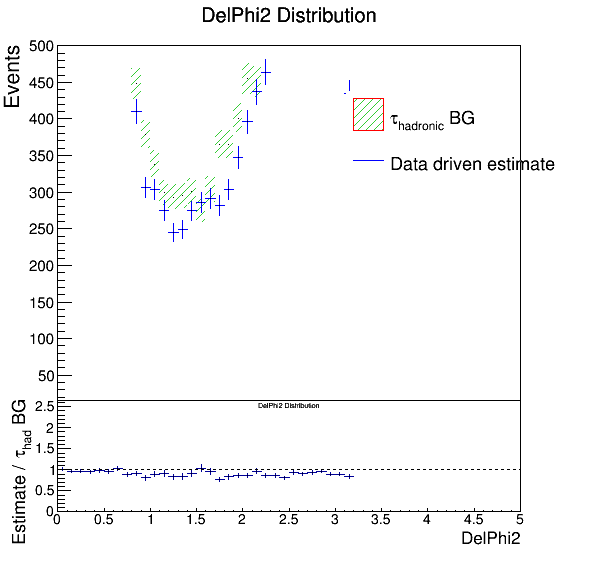
\includegraphics[width=1.\textwidth]{figures/HadTau/FromKen/DeltaPhi2_SimplifiedClosure1.png}};
    \begin{scope}[x={(image.south east)},y={(image.north west)}]
    \end{scope}
   \end{tikzpicture}
  \end{column}
  \begin{column}{0.33\textwidth}
   \begin{tikzpicture}
    \node[anchor=south west,inner sep=0] (image) at (0,0) {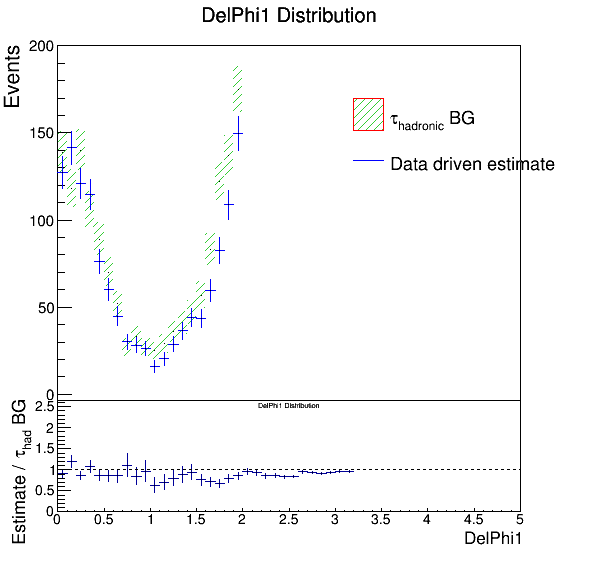
\includegraphics[width=1.\textwidth]{figures/HadTau/FromKen/DeltaPhi1_SimplifiedClosure1.png}};
    \begin{scope}[x={(image.south east)},y={(image.north west)}]
    \end{scope}
   \end{tikzpicture}
   \begin{tikzpicture}
    \node[anchor=south west,inner sep=0] (image) at (0,0) {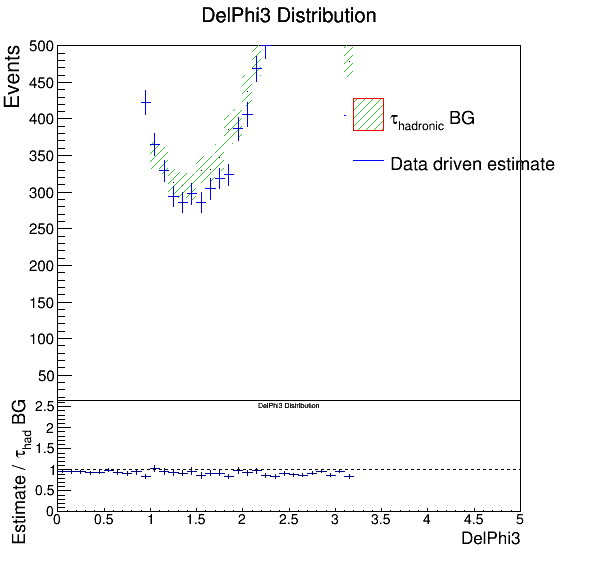
\includegraphics[width=1.\textwidth]{figures/HadTau/FromKen/DeltaPhi3_SimplifiedClosure1.png}};
    \begin{scope}[x={(image.south east)},y={(image.north west)}]
    \end{scope}
   \end{tikzpicture}
  \end{column}
 \end{columns}
\end{frame}

\begin{frame}
 \frametitle{Simplified Closure with $\Delta\phi(\MHT,j_{1,2,3})$}
 \begin{columns}
  \begin{column}{0.33\textwidth}
  \begin{itemize}
   \item $\Delta\phi(\MHT,j_{1})>0.5$
   \item $\Delta\phi(\MHT,j_{2})>0.5$
   \item $\Delta\phi(\MHT,j_{3})>0.3$ 
   \item Still 10\% non-closure, but closure is stable w.r.t. search variables
  \end{itemize}
  \end{column}
  \begin{column}{0.33\textwidth}
   \begin{tikzpicture}
    \node[anchor=south west,inner sep=0] (image) at (0,0) {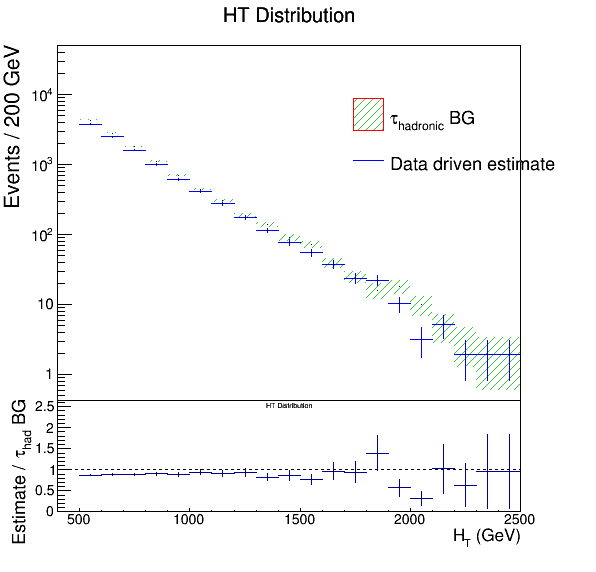
\includegraphics[width=1.\textwidth]{figures/HadTau/FromKen/HT_SimplifiedClosure2.png}};
    \begin{scope}[x={(image.south east)},y={(image.north west)}]
    \end{scope}
   \end{tikzpicture}
   \begin{tikzpicture}
    \node[anchor=south west,inner sep=0] (image) at (0,0) {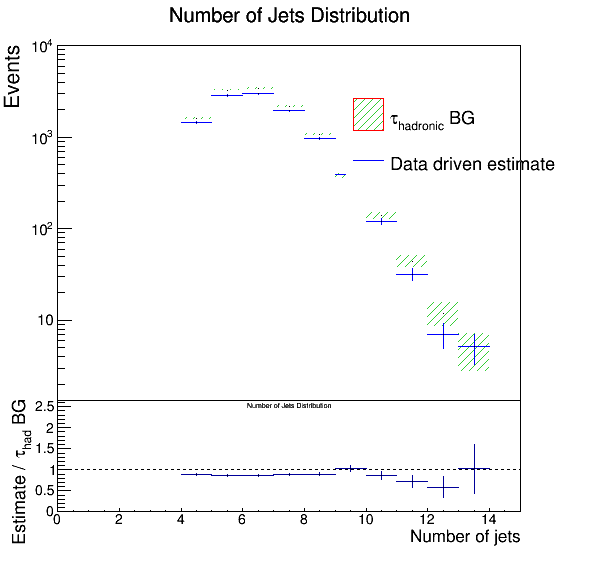
\includegraphics[width=1.\textwidth]{figures/HadTau/FromKen/NJets_SimplifiedClosure2.png}};
    \begin{scope}[x={(image.south east)},y={(image.north west)}]
    \end{scope}
   \end{tikzpicture}
  \end{column}
  \begin{column}{0.33\textwidth}
   \begin{tikzpicture}
    \node[anchor=south west,inner sep=0] (image) at (0,0) {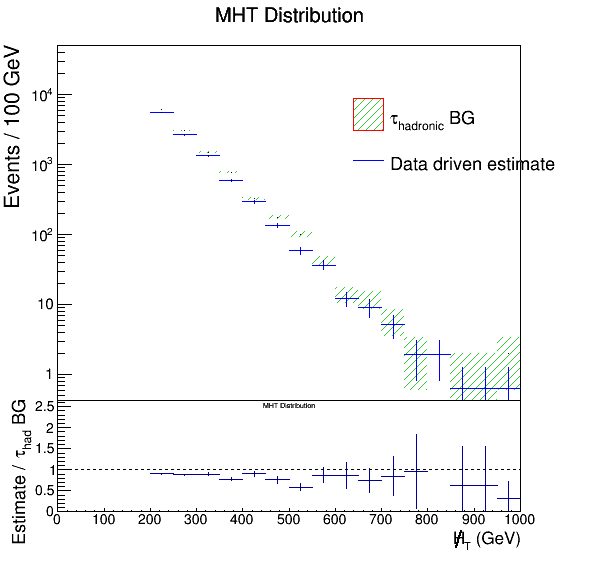
\includegraphics[width=1.\textwidth]{figures/HadTau/FromKen/MHT_SimplifiedClosure2.png}};
    \begin{scope}[x={(image.south east)},y={(image.north west)}]
    \end{scope}
   \end{tikzpicture}
   \begin{tikzpicture}
    \node[anchor=south west,inner sep=0] (image) at (0,0) {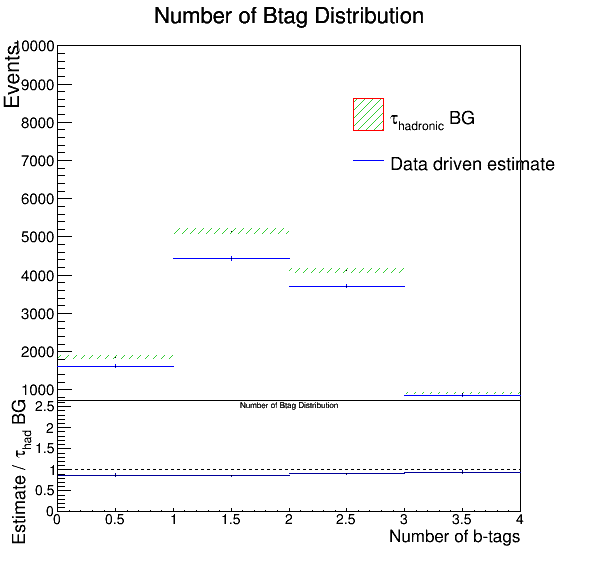
\includegraphics[width=1.\textwidth]{figures/HadTau/FromKen/BTags_SimplifiedClosure2.png}};
    \begin{scope}[x={(image.south east)},y={(image.north west)}]
    \end{scope}
   \end{tikzpicture}
  \end{column}
 \end{columns}
\end{frame}


\begin{frame}
 \frametitle{Adding back in $\tau\rightarrow\mu$ events}
 \begin{columns}
  \begin{column}{0.33\textwidth}
  \begin{itemize}
   \item Including now also $\tau\rightarrow\mu$ for the single $\mu$ control-sample
   \item $\Delta\phi(\MHT,j_{1,2,3})$ cut used
   \item Strong \HT dependency visible!
  \end{itemize}
  \end{column}
  \begin{column}{0.33\textwidth}
   \begin{tikzpicture}
    \node[anchor=south west,inner sep=0] (image) at (0,0) {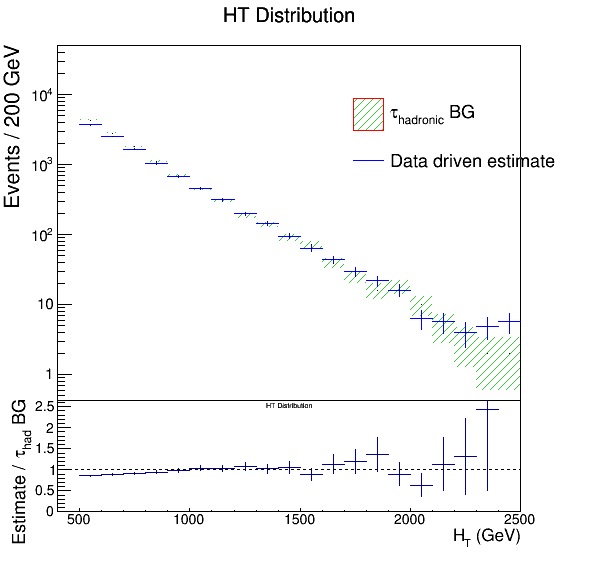
\includegraphics[width=1.\textwidth]{figures/HadTau/FromKen/HT_SimplifiedClosure3.png}};
    \begin{scope}[x={(image.south east)},y={(image.north west)}]
    \end{scope}
   \end{tikzpicture}
   \begin{tikzpicture}
    \node[anchor=south west,inner sep=0] (image) at (0,0) {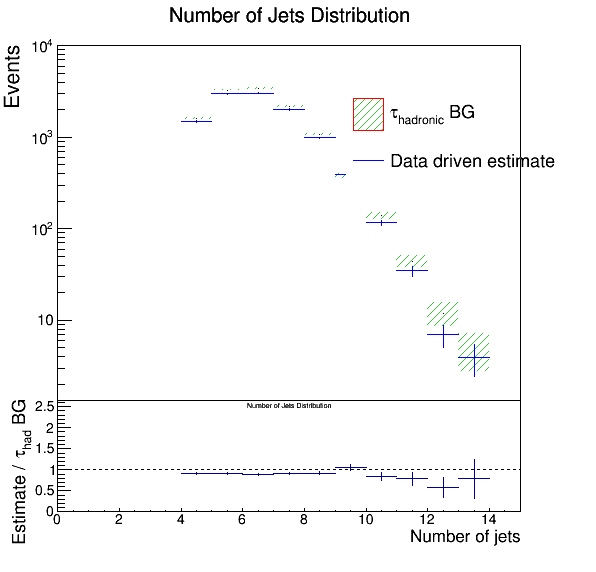
\includegraphics[width=1.\textwidth]{figures/HadTau/FromKen/NJets_SimplifiedClosure3.png}};
    \begin{scope}[x={(image.south east)},y={(image.north west)}]
    \end{scope}
   \end{tikzpicture}
  \end{column}
  \begin{column}{0.33\textwidth}
   \begin{tikzpicture}
    \node[anchor=south west,inner sep=0] (image) at (0,0) {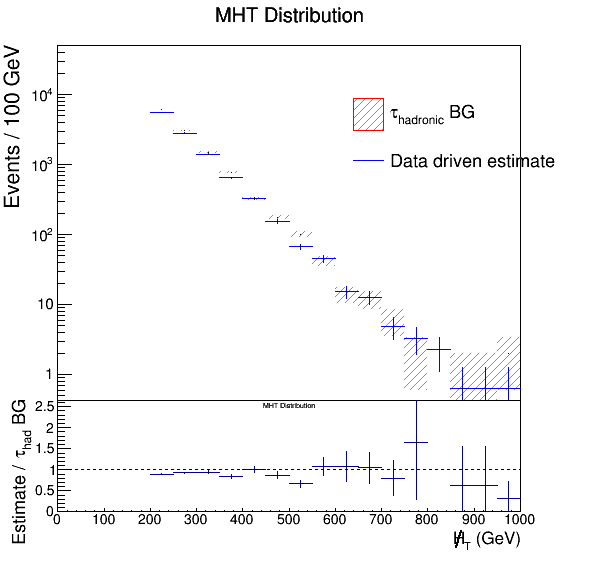
\includegraphics[width=1.\textwidth]{figures/HadTau/FromKen/MHT_SimplifiedClosure3.png}};
    \begin{scope}[x={(image.south east)},y={(image.north west)}]
    \end{scope}
   \end{tikzpicture}
   \begin{tikzpicture}
    \node[anchor=south west,inner sep=0] (image) at (0,0) {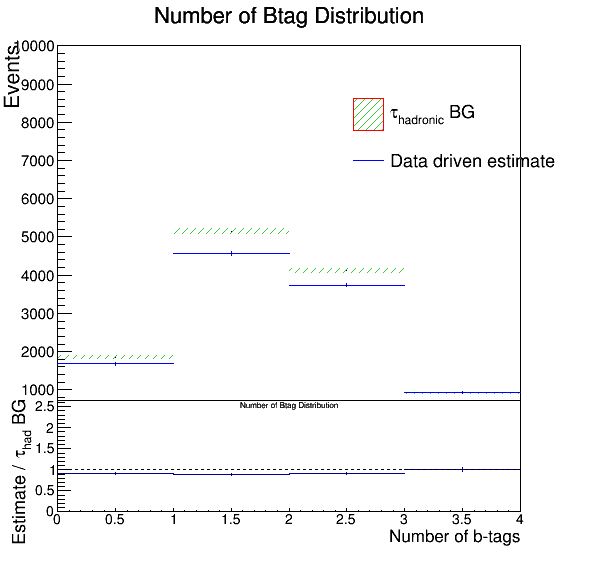
\includegraphics[width=1.\textwidth]{figures/HadTau/FromKen/BTags_SimplifiedClosure3.png}};
    \begin{scope}[x={(image.south east)},y={(image.north west)}]
    \end{scope}
   \end{tikzpicture}
  \end{column}
 \end{columns}
\end{frame}

\begin{frame}
 
 \begin{columns}
  \begin{column}{0.40\textwidth}
   \begin{itemize}
    \item Metod aims at using direct \wtomu events. 
    \item Reality includes \wtotautomu events
    \item Correcting as a function of $\mu$ \pt insuffiant
    \item Move to: 3D binning: \HT,\MHT\&\NJets
   \end{itemize}

  \end{column}
  \begin{column}{0.60\textwidth}
   \begin{tikzpicture}
    \node[anchor=south west,inner sep=0] (image) at (0,0) {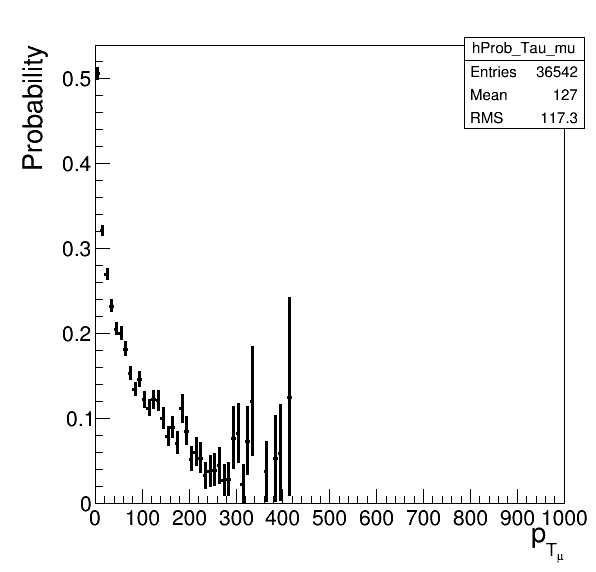
\includegraphics[width=.7\textwidth]{figures/HadTau/FromKen/TauToMuCorrectionFunctionOfPT.png}};
    \begin{scope}[x={(image.south east)},y={(image.north west)}]
    \end{scope}
   \end{tikzpicture}
   \begin{tikzpicture}
    \node[anchor=south west,inner sep=0] (image) at (0,0) {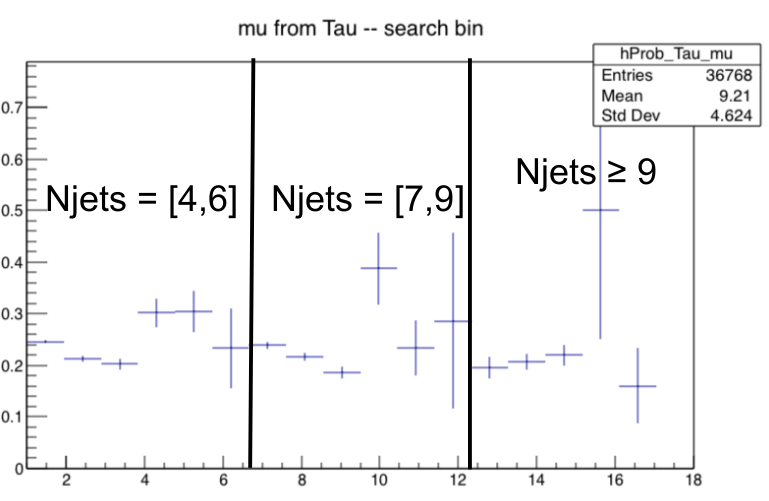
\includegraphics[width=.8\textwidth]{figures/HadTau/FromKen/CorrectionForTauToMuDecays.png}};
    \begin{scope}[x={(image.south east)},y={(image.north west)}]
    \end{scope}
   \end{tikzpicture}
  \end{column}
 \end{columns}

\end{frame}

\begin{frame}
%  \frametitle{Adding back in $\tau\rightarrow\mu$ events}
 \begin{columns}
  \begin{column}{0.33\textwidth}
  \begin{itemize}
   \item Correcting for $\tau\rightarrow\mu$ as a function of  \HT,\MHT\&\NJets resolves \HT dependency
  \end{itemize}
  \end{column}
  \begin{column}{0.33\textwidth}
   \begin{tikzpicture}
    \node[anchor=south west,inner sep=0] (image) at (0,0) {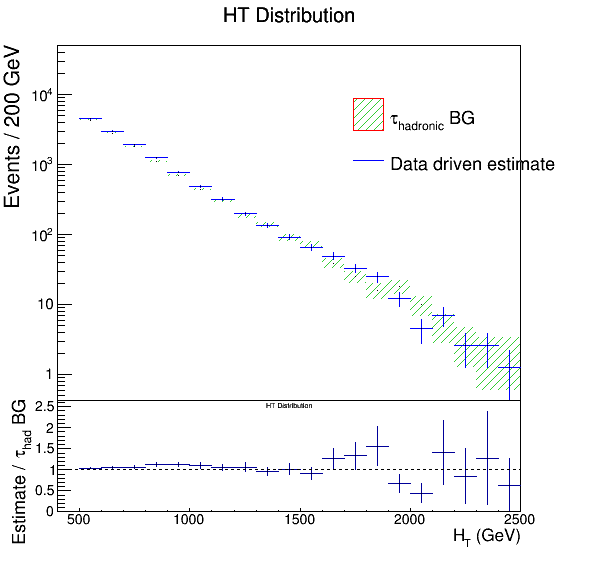
\includegraphics[width=1.\textwidth]{figures/HadTau/FromKen/HT_SimplifiedClosure4.png}};
    \begin{scope}[x={(image.south east)},y={(image.north west)}]
    \end{scope}
   \end{tikzpicture}
   \begin{tikzpicture}
    \node[anchor=south west,inner sep=0] (image) at (0,0) {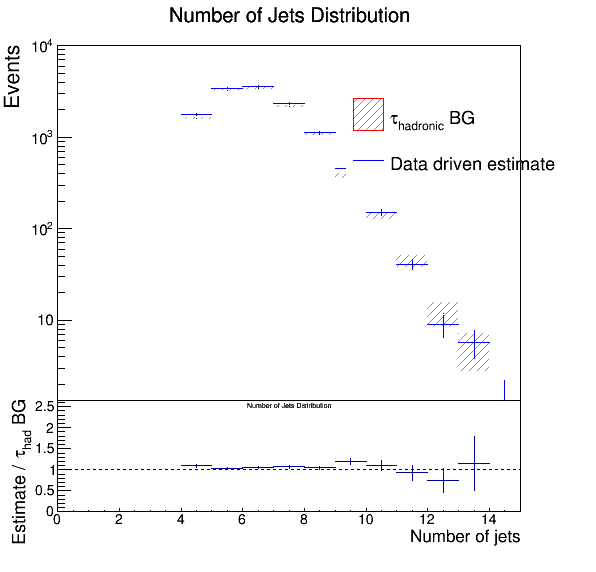
\includegraphics[width=1.\textwidth]{figures/HadTau/FromKen/NJets_SimplifiedClosure4.png}};
    \begin{scope}[x={(image.south east)},y={(image.north west)}]
    \end{scope}
   \end{tikzpicture}
  \end{column}
  \begin{column}{0.33\textwidth}
   \begin{tikzpicture}
    \node[anchor=south west,inner sep=0] (image) at (0,0) {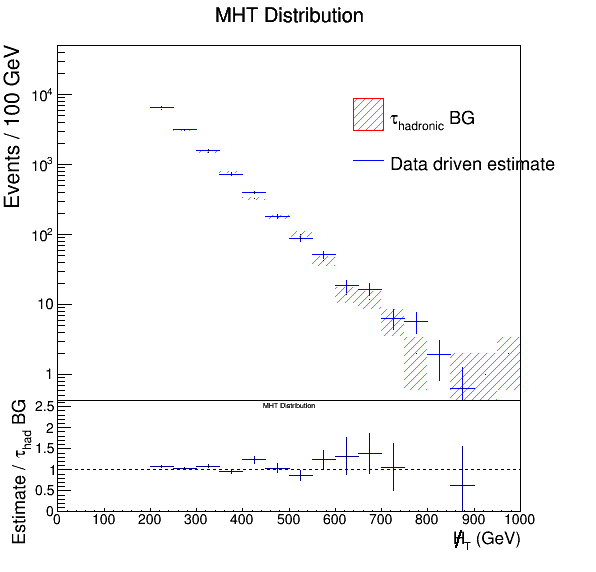
\includegraphics[width=1.\textwidth]{figures/HadTau/FromKen/MHT_SimplifiedClosure4.png}};
    \begin{scope}[x={(image.south east)},y={(image.north west)}]
    \end{scope}
   \end{tikzpicture}
   \begin{tikzpicture}
    \node[anchor=south west,inner sep=0] (image) at (0,0) {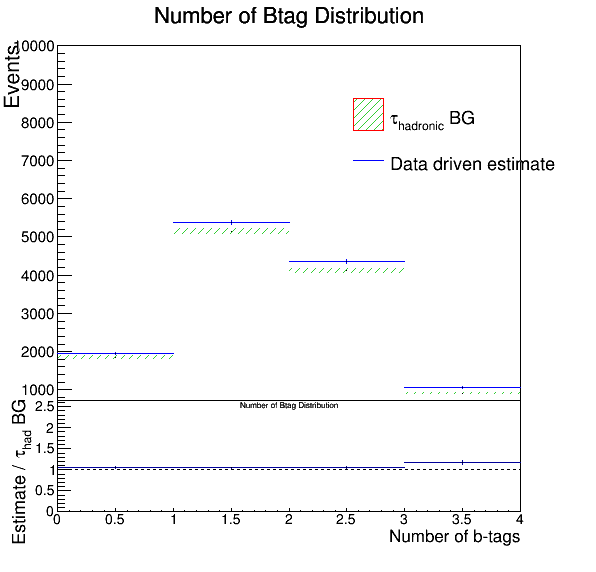
\includegraphics[width=1.\textwidth]{figures/HadTau/FromKen/BTags_SimplifiedClosure4.png}};
    \begin{scope}[x={(image.south east)},y={(image.north west)}]
    \end{scope}
   \end{tikzpicture}
  \end{column}
 \end{columns}
\end{frame}

\begin{frame}
 \frametitle{To Do List:}
 \begin{itemize}
  \item Reverting simplification steps, put in again:
  \begin{itemize}
   \item Lepton veto
   \item Use reconstructed \& isolated $\mu$ control sample
   \item Apply out of acceptance correction 
  \end{itemize}
  \item Merge effort by Rishi to scan entire template for each event to in crease precision  (bootstrap method)
  \item Include \wpj
  \item Include isolated track correction
 \end{itemize}
 
  \begin{block}{}
 \centering
 We will try to sort out most of these topics this week
 \end{block}
 

\end{frame}



\begin{frame}
 \begin{block}{}
 \centering
 \Large Backup
 \end{block}
\end{frame}

\section{Tag \& Probe}
\subsection{Setup: Leptons}
\begin{frame}
%  \frametitle{Mini Isolation (UCSB approach \href{https://indico.cern.ch/event/368826/contribution/3/material/slides/0.pdf}{Adam talk}) vs Classical Isolation}
\frametitle{Electron Muon Lepton Tag \& Probe Setup }
\begin{itemize}
 \item Muon:
 \begin{itemize}
  \item Reco/ID: "Tight" ID, $\pt>10 GeV$, $|\eta|<2.4$
  \item Iso: Mini Isolation: Max Cone: 0.2 Min Cone: 0.05 $\delta \beta I(rel)<0.2$
 \end{itemize}
  \item Electron:
 \begin{itemize}
  \item Reco/ID: "Veto" ID, $\pt>10 GeV$, $|\eta|<2.5$
  \item Iso: Mini Isolation: Max Cone: 0.2 Min Cone: 0.05 $\delta \beta I(rel)<0.1$
 \end{itemize}
 \item Tag \& Probe:
 \begin{itemize}
  \item Tag: Isolated $\mu$/e (high purity RA2b definition)
 \item ID:  (problematic direct comparison to eff from \ttbar \& \wpj)
 \begin{itemize}
  \item Problem: ChargedPFCands(slimmedPhotons) $\rightarrow$ Reco\&ID muon(electron)
  \item Problem: Muons: chargedPFCands, bad ratio signal / background, electron: slimmedPhotons miniAOD stores only down to 14 GeV $\rightarrow$ use AOD (not done)
 \end{itemize}
  \item Iso: (directly comparable to eff from \ttbar \& \wpj)
 \begin{itemize}
  \item Tag: Iso muon(Electron)
  \item Probe: Reco/ID muon(electron) $\rightarrow$ Iso muon(electron)
 
 \end{itemize}

 \end{itemize}
\end{itemize}
\end{frame}


% \begin{frame}
%  \frametitle{Tag \& Probe technicals}
%  \begin{itemize}
%   \item Test Several cuts to increase kinetically similarity to search region
%   \begin{itemize}
%    \item $\HT>500,400,200 \gev$
%    \item $\mindeltaphi >4.0, No Cut$ (Treat Tag leptons \pt as neutrino \pt $\rightarrow$ \MHT)
%    \item $\NJets\geq4$
%   \end{itemize}
%
%   \item Apply $\HT>500$ \& $\NJets\geq4$ (similar kinematics to baseline region)
%   \item Select (randomly) tag lepton from isolated lepton collection
%   \item Select all probe leptons except matched to tag
%   \item Compute for all invariant mass (Z mass)
%   \item Check property (ID/iso criteria)
%   \item Use electroweak code for fitting and eff. determination
%   \begin{itemize}
%    \item Fit function: gaussPlusCubic
%   \end{itemize}
%
%  \end{itemize}
% \end{frame}
\subsection{$\mu$ Efficiencies}
\begin{frame}
 \begin{block}{}
 \centering
 \Large Tag \& Probe $\mu$ Isolation/Reconstruction Efficiencies
 \end{block}
\end{frame}

\begin{frame}
 \frametitle{Comparison \ttbar \& \wpj vs DY Tag \& Probe $\mu$ Iso Efficiencies}
   \begin{columns}

   \begin{column}{0.33\textwidth}
     \begin{itemize}
   \item $\mu$ Iso \ttbar \& \wpj eff. (truth info.)
  \end{itemize}
    \begin{tikzpicture}
    \node[anchor=south west,inner sep=0] (image) at (0,0) {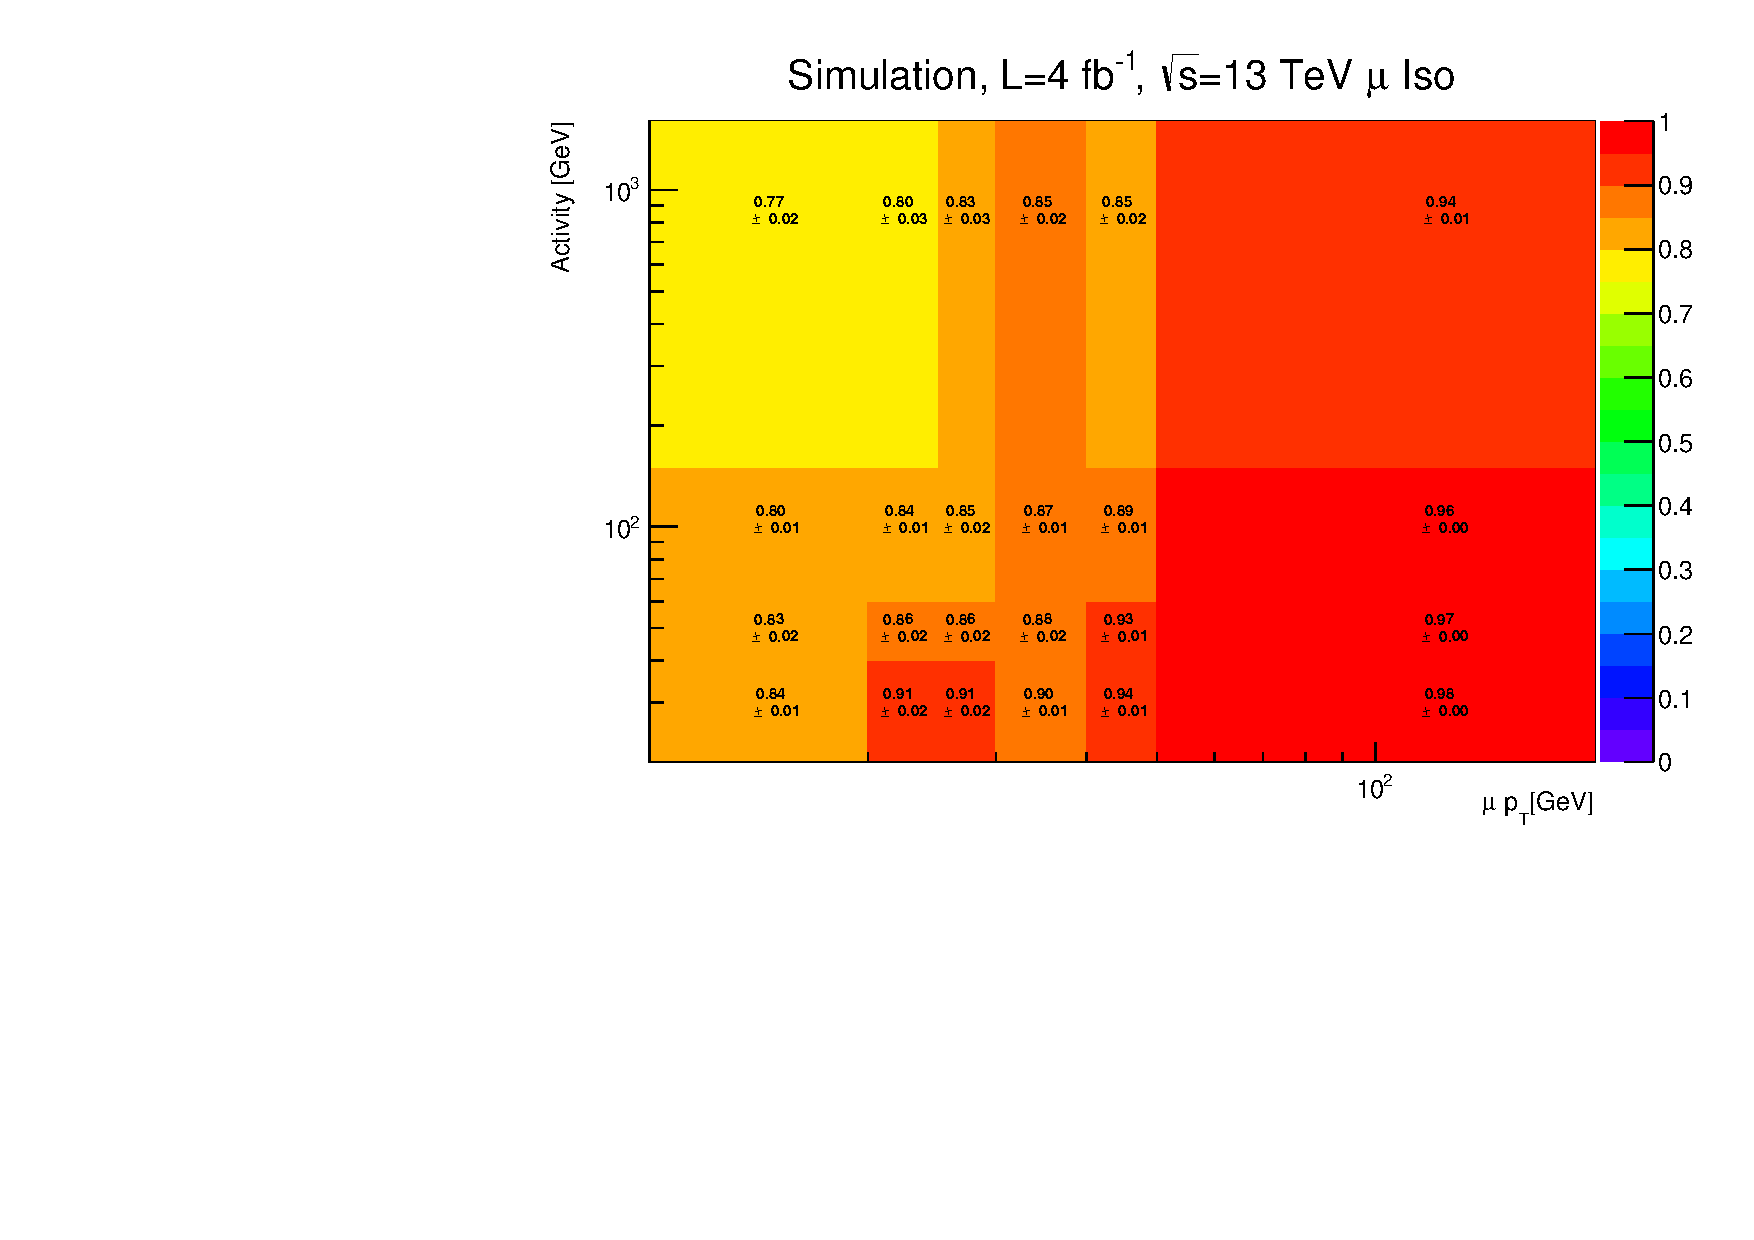
\includegraphics[width=1.\textwidth]{figures/Efficiencies/oldJEC/ttbarwpjTruth/MuIsoPTActivity.pdf}};
    \begin{scope}[x={(image.south east)},y={(image.north west)}]
%         \draw[red,ultra thick,rounded corners] (0.62,0.65) rectangle (0.78,0.75);
%         \draw[red,ultra thick,rounded corners] (0.60,0.01) rectangle (0.75,0.99); % coordinates unten links(x,y) oben rechts(x,y)
    \end{scope}
   \end{tikzpicture}
   \end{column}
   \begin{column}{0.33\textwidth}
   \begin{itemize}
    \item $\mu$ Iso DY eff. \\(Tag \& Probe)
   \end{itemize}

    \begin{tikzpicture}
    \node[anchor=south west,inner sep=0] (image) at (0,0) {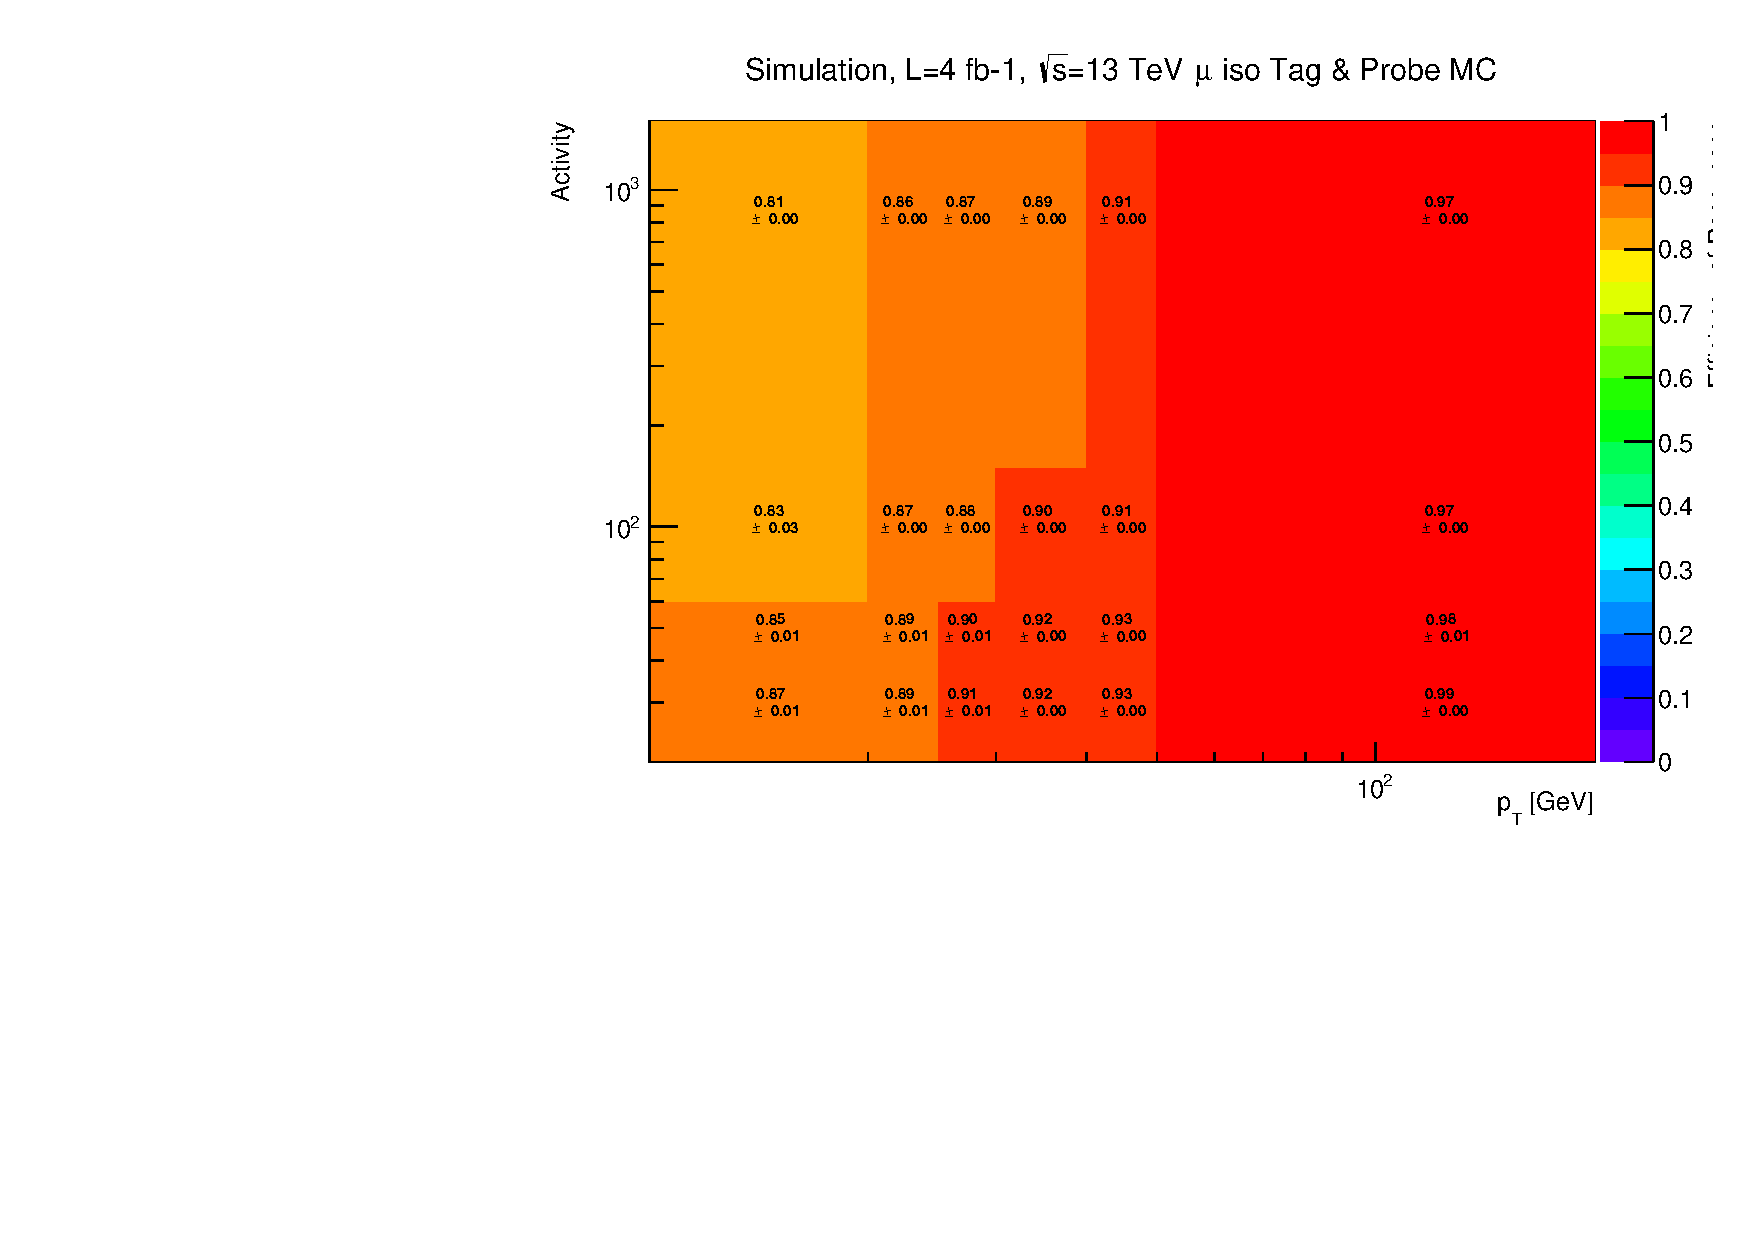
\includegraphics[width=1.\textwidth]{figures/Efficiencies/oldJEC/tagAndProbe/MuIsoTagAndProbeMC.pdf}};
    \begin{scope}[x={(image.south east)},y={(image.north west)}]
%         \draw[red,ultra thick,rounded corners] (0.62,0.65) rectangle (0.78,0.75);
%         \draw[red,ultra thick,rounded corners] (0.60,0.01) rectangle (0.75,0.99); % coordinates unten links(x,y) oben rechts(x,y)
    \end{scope}
   \end{tikzpicture}
   \end{column}
           \begin{column}{0.33\textwidth}
   \begin{itemize}
    \item $\mu$ iso radio
   \end{itemize}

    \begin{tikzpicture}
     \node[anchor=south west,inner sep=0] (image) at (0,0) {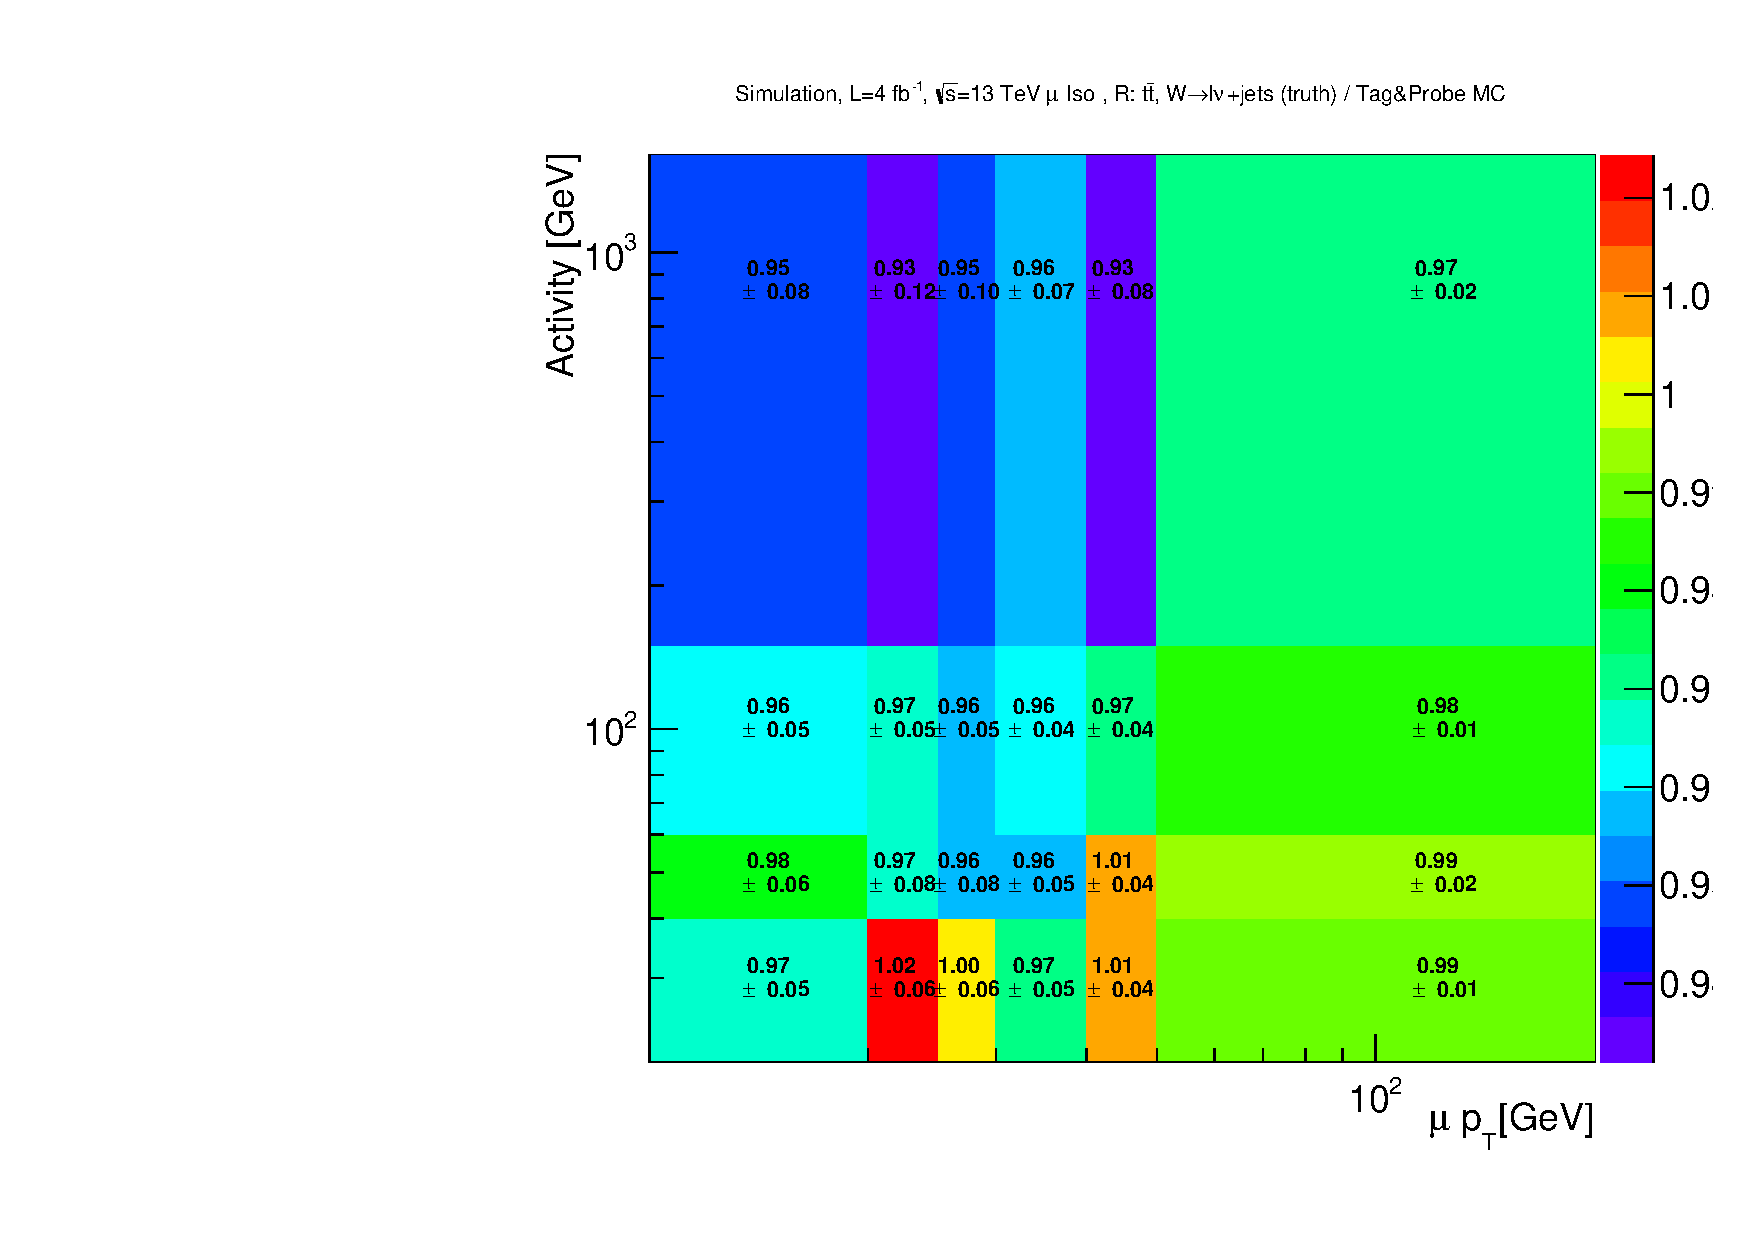
\includegraphics[width=1.\textwidth]{figures/Efficiencies/oldJEC/tagAndProbe/MuIsoPTActivity_ratio.pdf}};
    \begin{scope}[x={(image.south east)},y={(image.north west)}]
%         \draw[red,ultra thick,rounded corners] (0.62,0.65) rectangle (0.78,0.75);
%         \draw[red,ultra thick,rounded corners] (0.60,0.01) rectangle (0.75,0.99); % coordinates unten links(x,y) oben rechts(x,y)
    \end{scope}
   \end{tikzpicture}
   \end{column}
  \end{columns}
\begin{itemize}
 \item Efficiencies obtained (using truth information) from \ttbar \& \wpj and DY are in good agreement
 \item Lepton \pt and Activity are sufficient topology independent to be transfered from DY to signal region! (Confirm Florent)
 \item Overall the efficiencies from DY are slightly higher. (No cuts applied to DY \ttbar \& \wpj baseline applied)
\end{itemize}
\end{frame}

\begin{frame}
 \frametitle{Comparison \ttbar \& \wpj vs DY-Truth $\mu$ Reco Efficiencies}
  \begin{columns}

   \begin{column}{0.33\textwidth}
     \begin{itemize}
   \item $\mu$ ID \ttbar \& \wpj eff. (truth info.)
  \end{itemize}
    \begin{tikzpicture}
    \node[anchor=south west,inner sep=0] (image) at (0,0) {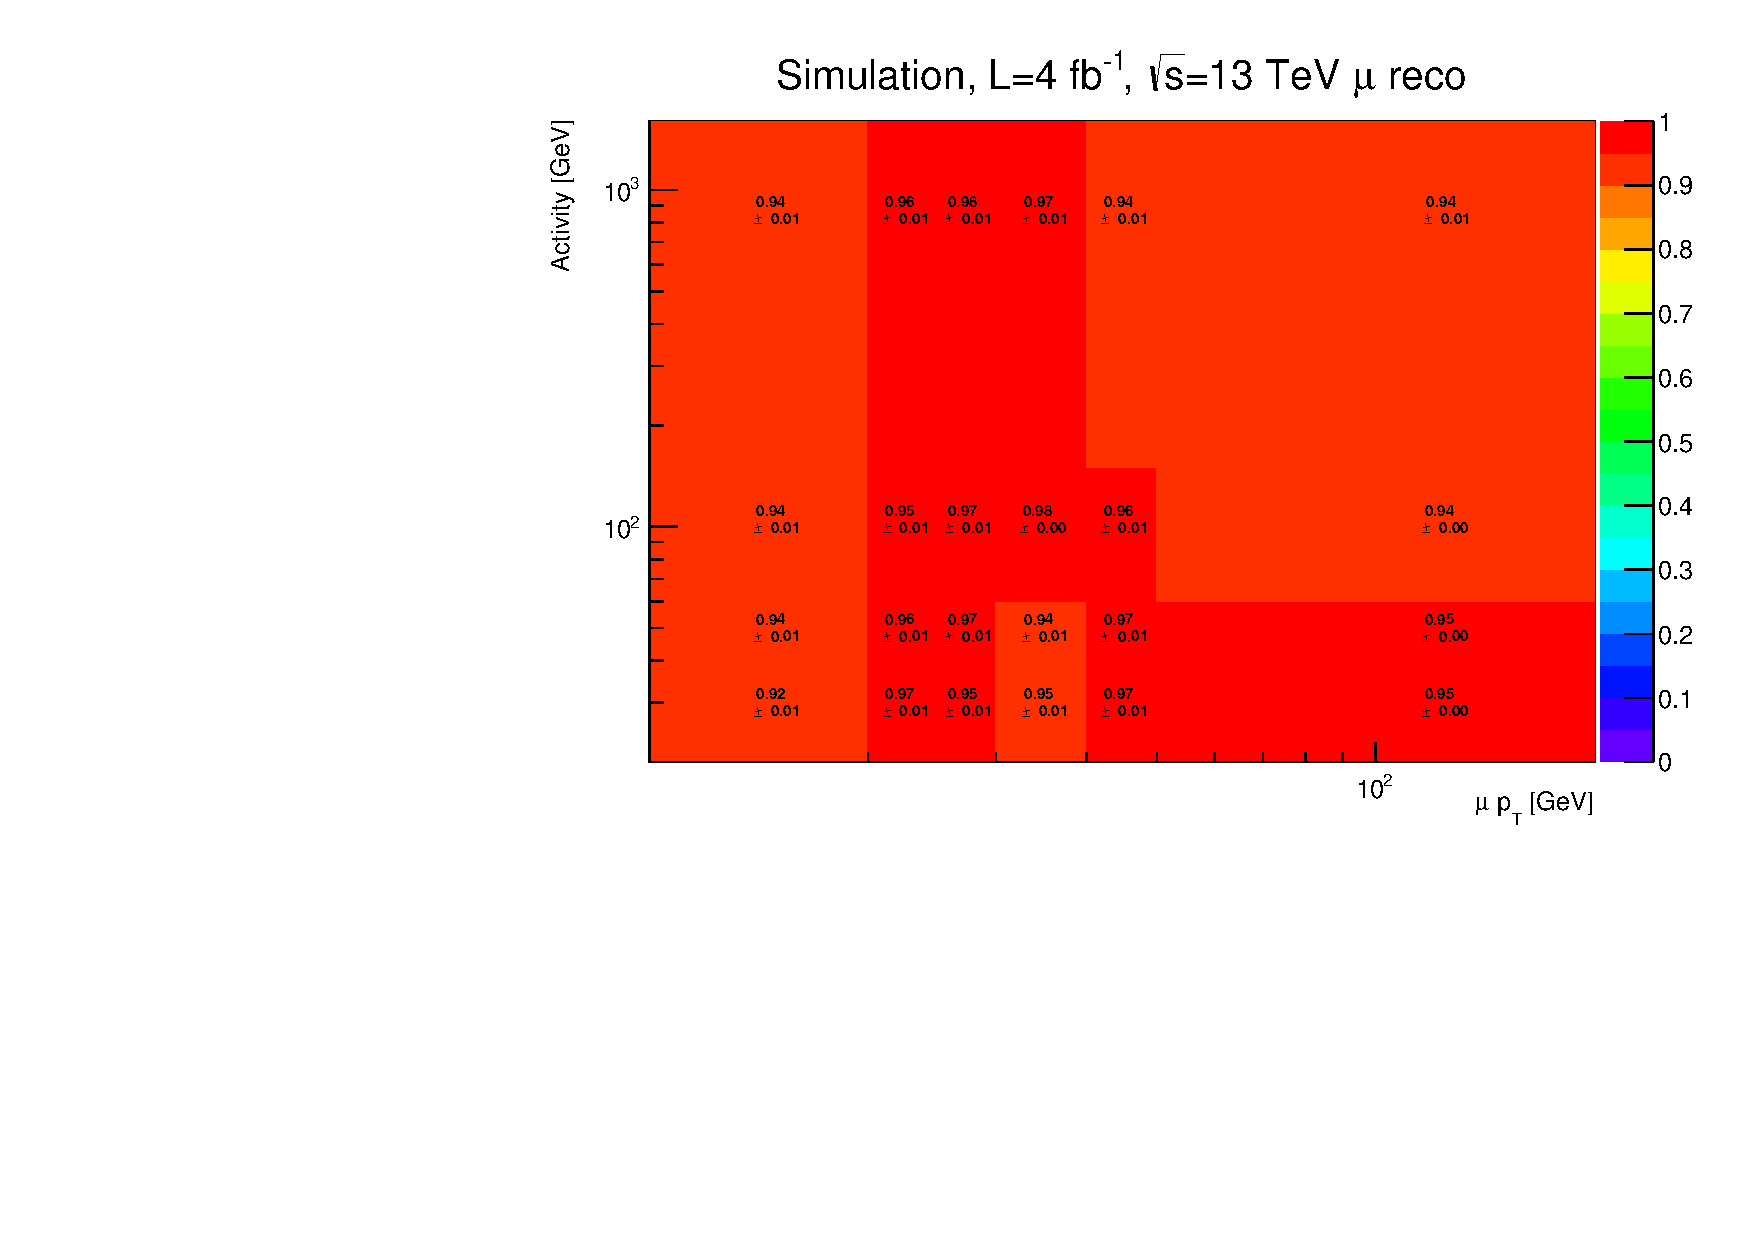
\includegraphics[width=1.\textwidth]{figures/Efficiencies/oldJEC/ttbarwpjTruth/MuRecoPTActivity.pdf}};
    \begin{scope}[x={(image.south east)},y={(image.north west)}]
%         \draw[red,ultra thick,rounded corners] (0.62,0.65) rectangle (0.78,0.75);
%         \draw[red,ultra thick,rounded corners] (0.60,0.01) rectangle (0.75,0.99); % coordinates unten links(x,y) oben rechts(x,y)
    \end{scope}
   \end{tikzpicture}
   \end{column}
   \begin{column}{0.33\textwidth}
   \begin{itemize}
    \item $\mu$ ID DY eff.\\ (truth info.)
   \end{itemize}

    \begin{tikzpicture}
     \node[anchor=south west,inner sep=0] (image) at (0,0) {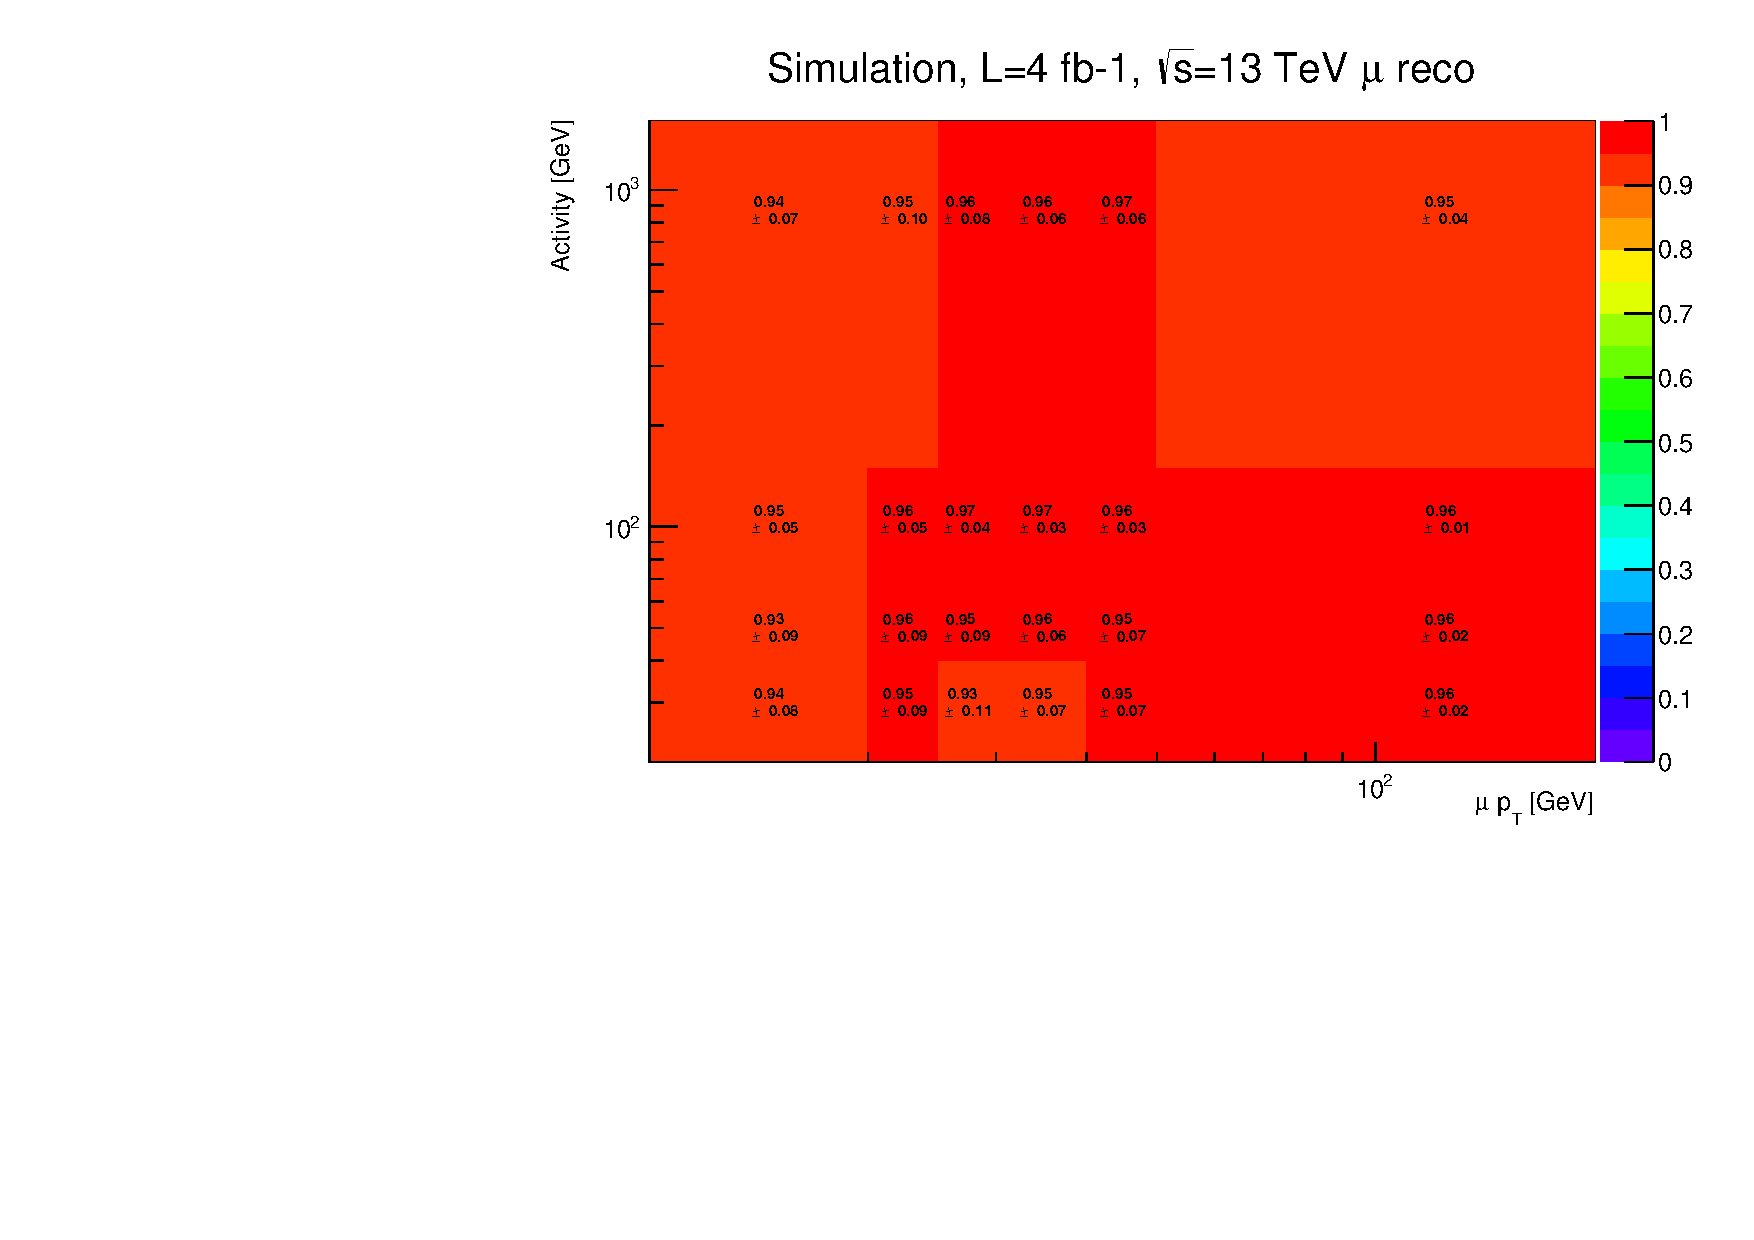
\includegraphics[width=1.\textwidth]{figures/Efficiencies/oldJEC/dytruth/MuRecoPTActivity_DY_noTagAndProbe.pdf}};
    \begin{scope}[x={(image.south east)},y={(image.north west)}]
%         \draw[red,ultra thick,rounded corners] (0.62,0.65) rectangle (0.78,0.75);
%         \draw[red,ultra thick,rounded corners] (0.60,0.01) rectangle (0.75,0.99); % coordinates unten links(x,y) oben rechts(x,y)
    \end{scope}
   \end{tikzpicture}
   \end{column}
        \begin{column}{0.33\textwidth}
   \begin{itemize}
    \item $\mu$ ID Tag \& Probe eff.
   \end{itemize}

    \begin{tikzpicture}
     \node[anchor=south west,inner sep=0] (image) at (0,0) {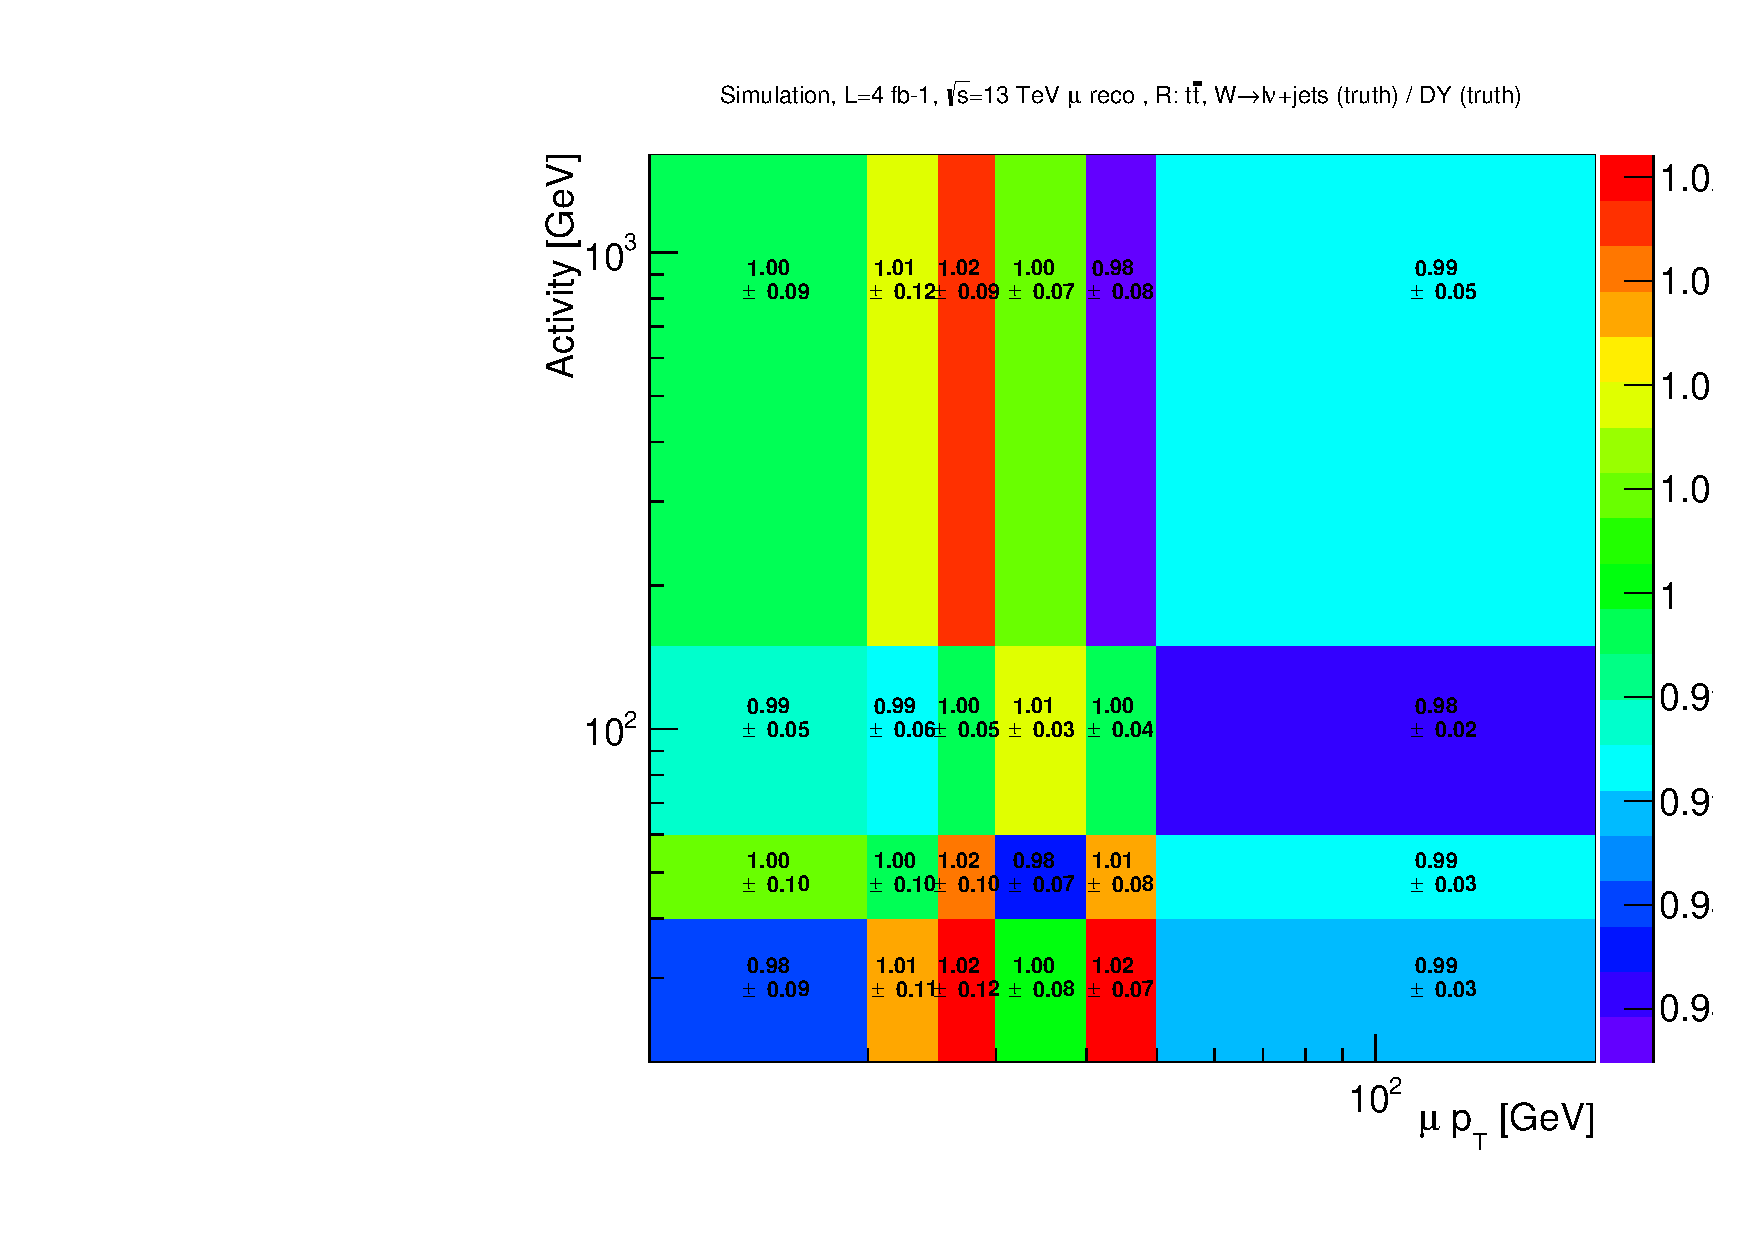
\includegraphics[width=1.\textwidth]{figures/Efficiencies/oldJEC/compareDYTruth_TTbarWPJTruth/MuRecoPTActivity_ratio.pdf}};
    \begin{scope}[x={(image.south east)},y={(image.north west)}]
%         \draw[red,ultra thick,rounded corners] (0.62,0.65) rectangle (0.78,0.75);
%         \draw[red,ultra thick,rounded corners] (0.60,0.01) rectangle (0.75,0.99); % coordinates unten links(x,y) oben rechts(x,y)
    \end{scope}
   \end{tikzpicture}
   \end{column}
  \end{columns}
\begin{itemize}
 \item Efficiencies obtained (using truth information) from \ttbar \& \wpj and DY are in good agreement.
 \item \ttbar \& \wpj eff. matching from all in acceptance (gen lepton) including non reco leptons
 \item \Zll eff. start with chargedPFCands/slimmedPhotons (slimmedMuon/slimmedElectron) (non reco excluded only test for ID)
\end{itemize}

\end{frame}


\begin{frame}
 \frametitle{Comparison \ttbar \& \wpj vs DY Tag \& Probe $\mu$ Reco Efficiencies}
   \begin{columns}

   \begin{column}{0.33\textwidth}
     \begin{itemize}
   \item $\mu$ Reco \ttbar \& \wpj eff. (truth info.)
  \end{itemize}
    \begin{tikzpicture}
    \node[anchor=south west,inner sep=0] (image) at (0,0) {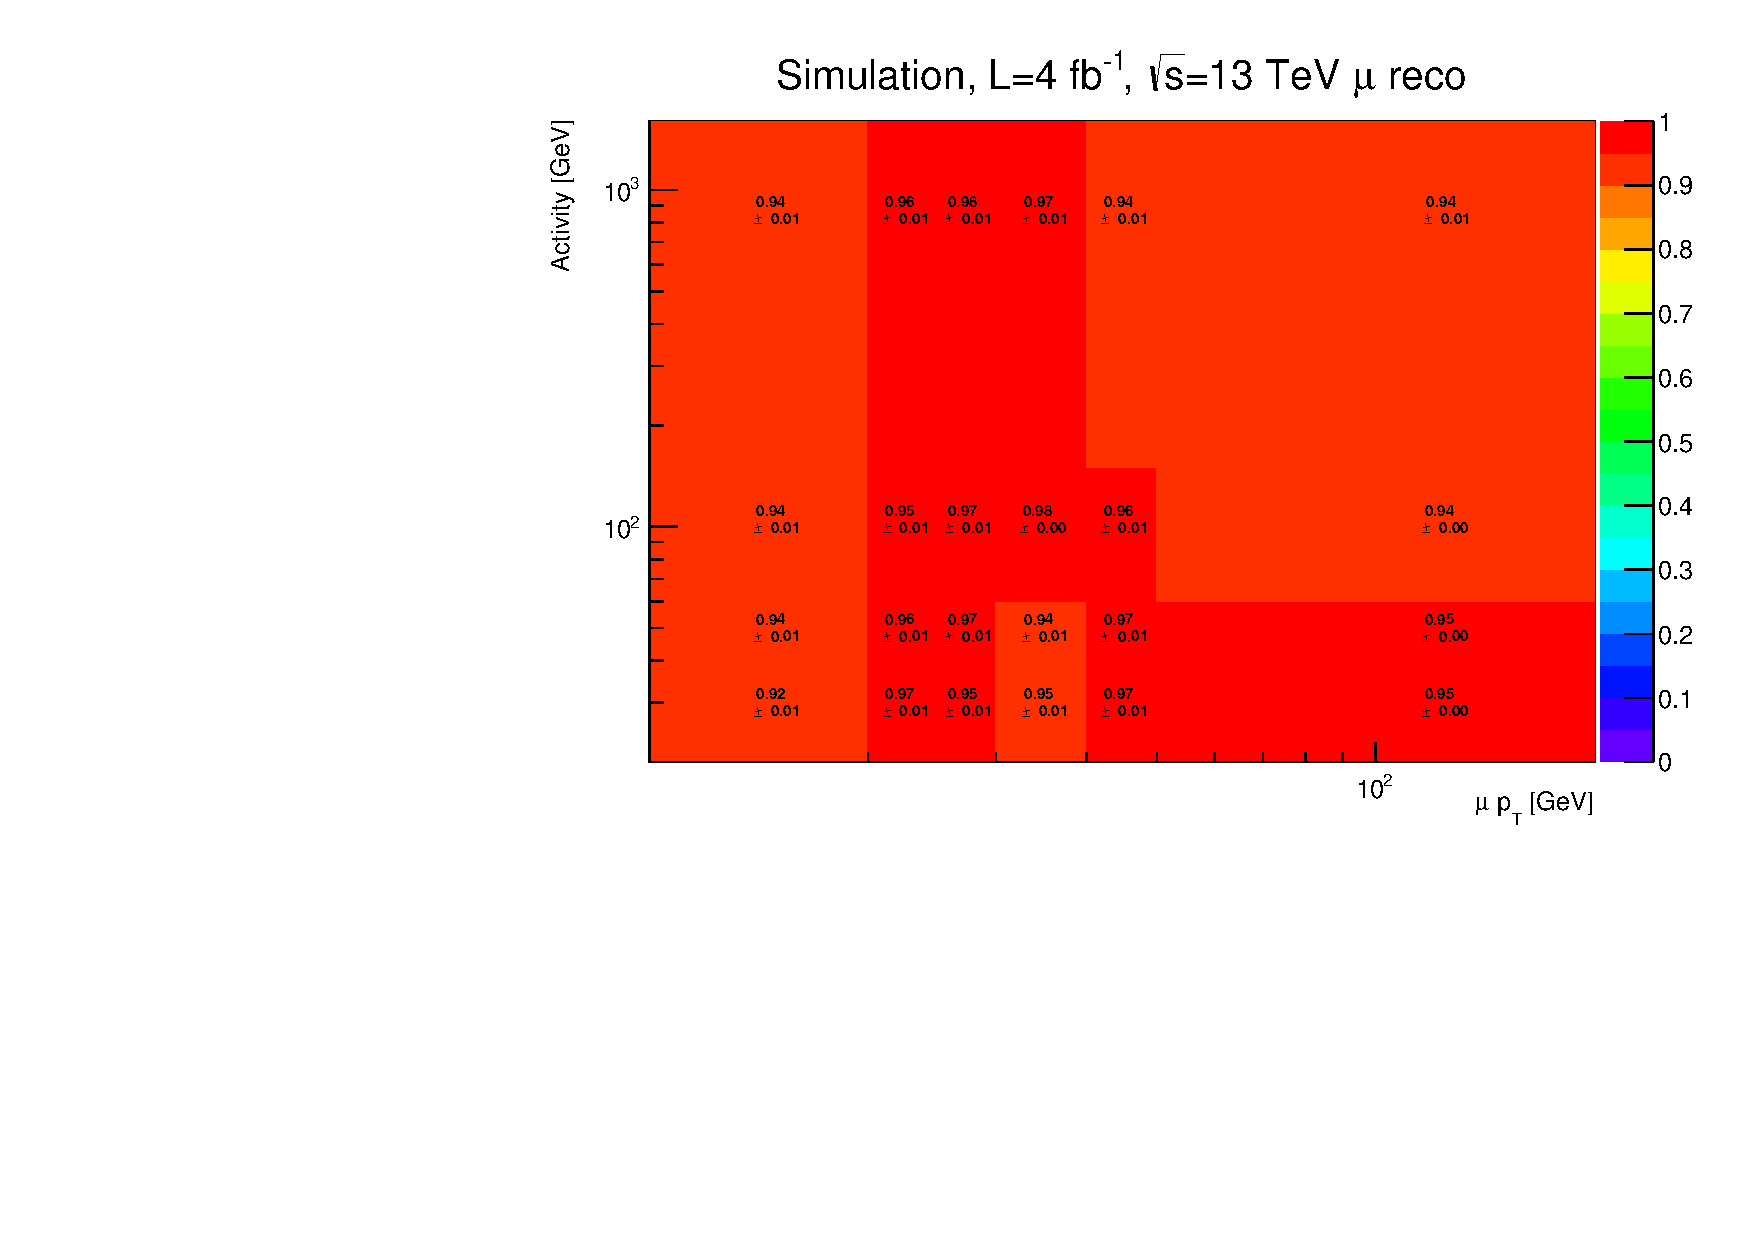
\includegraphics[width=1.\textwidth]{figures/Efficiencies/oldJEC/ttbarwpjTruth/MuRecoPTActivity.pdf}};
    \begin{scope}[x={(image.south east)},y={(image.north west)}]
%         \draw[red,ultra thick,rounded corners] (0.62,0.65) rectangle (0.78,0.75);
%         \draw[red,ultra thick,rounded corners] (0.60,0.01) rectangle (0.75,0.99); % coordinates unten links(x,y) oben rechts(x,y)
    \end{scope}
   \end{tikzpicture}
   \end{column}
   \begin{column}{0.33\textwidth}
   \begin{itemize}
    \item $\mu$ Reco DY eff. \\(Tag \& Probe)
   \end{itemize}

    \begin{tikzpicture}
    \node[anchor=south west,inner sep=0] (image) at (0,0) {\includegraphics[width=1.\textwidth]{figures/Efficiencies/oldJEC/tagAndProbe/MuRecoTagAndProbeMC.pdf}};
    \begin{scope}[x={(image.south east)},y={(image.north west)}]
%         \draw[red,ultra thick,rounded corners] (0.62,0.65) rectangle (0.78,0.75);
%         \draw[red,ultra thick,rounded corners] (0.60,0.01) rectangle (0.75,0.99); % coordinates unten links(x,y) oben rechts(x,y)
    \end{scope}
   \end{tikzpicture}
   \end{column}
           \begin{column}{0.33\textwidth}
   \begin{itemize}
    \item $\mu$ Reco radio
   \end{itemize}

    \begin{tikzpicture}
     \node[anchor=south west,inner sep=0] (image) at (0,0) {\includegraphics[width=1.\textwidth]{figures/Efficiencies/oldJEC/tagAndProbe/MuRecoPTActivity_ratio.pdf}};
    \begin{scope}[x={(image.south east)},y={(image.north west)}]
%         \draw[red,ultra thick,rounded corners] (0.62,0.65) rectangle (0.78,0.75);
%         \draw[red,ultra thick,rounded corners] (0.60,0.01) rectangle (0.75,0.99); % coordinates unten links(x,y) oben rechts(x,y)
    \end{scope}
   \end{tikzpicture}
   \end{column}
  \end{columns}
\begin{itemize}
 \item Starting from probe charged pfCand too high background to signal event ratio in failing. (Here only DY sample used full SM process a lot higher background)
 \item Need to apply more cuts on probe to achieve higher purity. (follow official approach)
\end{itemize}
\end{frame}
\subsection{e Efficiencies}
\begin{frame}
 \begin{block}{}
 \centering
 \Large Tag \& Probe e Efficiencies
 \end{block}
\end{frame}


\begin{frame}
 \frametitle{Comparison \ttbar \& \wpj vs DY Tag \& Probe e Iso Efficiencies}
   \begin{columns}

   \begin{column}{0.33\textwidth}
     \begin{itemize}
   \item e Iso \ttbar \& \wpj eff. (truth info.)
  \end{itemize}
    \begin{tikzpicture}
    \node[anchor=south west,inner sep=0] (image) at (0,0) {\includegraphics[width=1.\textwidth]{figures/Efficiencies/oldJEC/ttbarwpjTruth/ElecIsoPTActivity.pdf}};
    \begin{scope}[x={(image.south east)},y={(image.north west)}]
%         \draw[red,ultra thick,rounded corners] (0.62,0.65) rectangle (0.78,0.75);
%         \draw[red,ultra thick,rounded corners] (0.60,0.01) rectangle (0.75,0.99); % coordinates unten links(x,y) oben rechts(x,y)
    \end{scope}
   \end{tikzpicture}
   \end{column}
   \begin{column}{0.33\textwidth}
   \begin{itemize}
    \item e Iso DY eff. \\(Tag \& Probe)
   \end{itemize}

    \begin{tikzpicture}
    \node[anchor=south west,inner sep=0] (image) at (0,0) {\includegraphics[width=1.\textwidth]{figures/Efficiencies/oldJEC/tagAndProbe/ElecIsoTagAndProbeMC.pdf}};
    \begin{scope}[x={(image.south east)},y={(image.north west)}]
%         \draw[red,ultra thick,rounded corners] (0.62,0.65) rectangle (0.78,0.75);
%         \draw[red,ultra thick,rounded corners] (0.60,0.01) rectangle (0.75,0.99); % coordinates unten links(x,y) oben rechts(x,y)
    \end{scope}
   \end{tikzpicture}
   \end{column}
           \begin{column}{0.33\textwidth}
   \begin{itemize}
    \item e iso radio
   \end{itemize}

    \begin{tikzpicture}
     \node[anchor=south west,inner sep=0] (image) at (0,0) {\includegraphics[width=1.\textwidth]{figures/Efficiencies/oldJEC/tagAndProbe/ElecIsoPTActivity_ratio.pdf}};
    \begin{scope}[x={(image.south east)},y={(image.north west)}]
%         \draw[red,ultra thick,rounded corners] (0.62,0.65) rectangle (0.78,0.75);
%         \draw[red,ultra thick,rounded corners] (0.60,0.01) rectangle (0.75,0.99); % coordinates unten links(x,y) oben rechts(x,y)
    \end{scope}
   \end{tikzpicture}
   \end{column}
  \end{columns}
\begin{itemize}
 \item Efficiencies obtained (using truth information) from \ttbar \& \wpj and DY are in good agreement
 \item Lepton \pt and Activity are sufficient topology independent to be transfered from DY to signal region! (Confirm Florent)
 \item Overall the efficiencies from DY are slightly higher. (No cuts applied to DY \ttbar \& \wpj baseline applied)
\end{itemize}
\end{frame}

\begin{frame}
 \frametitle{Comparison \ttbar \& \wpj vs DY-Truth e Reco Efficiencies}
  \begin{columns}

   \begin{column}{0.33\textwidth}
     \begin{itemize}
   \item e ID \ttbar \& \wpj eff. (truth info.)
  \end{itemize}
    \begin{tikzpicture}
    \node[anchor=south west,inner sep=0] (image) at (0,0) {\includegraphics[width=1.\textwidth]{figures/Efficiencies/oldJEC/ttbarwpjTruth/ElecRecoPTActivity.pdf}};
    \begin{scope}[x={(image.south east)},y={(image.north west)}]
%         \draw[red,ultra thick,rounded corners] (0.62,0.65) rectangle (0.78,0.75);
%         \draw[red,ultra thick,rounded corners] (0.60,0.01) rectangle (0.75,0.99); % coordinates unten links(x,y) oben rechts(x,y)
    \end{scope}
   \end{tikzpicture}
   \end{column}
   \begin{column}{0.33\textwidth}
   \begin{itemize}
    \item e ID DY eff.\\ (truth info.)
   \end{itemize}

    \begin{tikzpicture}
     \node[anchor=south west,inner sep=0] (image) at (0,0) {\includegraphics[width=1.\textwidth]{figures/Efficiencies/oldJEC/dytruth/ElecRecoPTActivity_DY_noTagAndProbe.pdf}};
    \begin{scope}[x={(image.south east)},y={(image.north west)}]
%         \draw[red,ultra thick,rounded corners] (0.62,0.65) rectangle (0.78,0.75);
%         \draw[red,ultra thick,rounded corners] (0.60,0.01) rectangle (0.75,0.99); % coordinates unten links(x,y) oben rechts(x,y)
    \end{scope}
   \end{tikzpicture}
   \end{column}
        \begin{column}{0.33\textwidth}
   \begin{itemize}
    \item e ID Tag \& Probe eff.
   \end{itemize}

    \begin{tikzpicture}
     \node[anchor=south west,inner sep=0] (image) at (0,0) {\includegraphics[width=1.\textwidth]{figures/Efficiencies/oldJEC/compareDYTruth_TTbarWPJTruth/ElecRecoPTActivity_ratio.pdf}};
    \begin{scope}[x={(image.south east)},y={(image.north west)}]
%         \draw[red,ultra thick,rounded corners] (0.62,0.65) rectangle (0.78,0.75);
%         \draw[red,ultra thick,rounded corners] (0.60,0.01) rectangle (0.75,0.99); % coordinates unten links(x,y) oben rechts(x,y)
    \end{scope}
   \end{tikzpicture}
   \end{column}
  \end{columns}
\begin{itemize}
 \item Efficiencies obtained (using truth information) from \ttbar \& \wpj and DY are in good agreement.
 \item \ttbar \& \wpj eff. matching from all in acceptance (gen lepton) including non reco leptons
 \item \Zll eff. start with chargedPFCands/slimmedPhotons (slimmedElecon/slimmedElectron) (non reco excluded only test for ID)
\end{itemize}

\end{frame}


\begin{frame}
 \frametitle{Comparison \ttbar \& \wpj vs DY Tag \& Probe e Reco Efficiencies}
   \begin{columns}

   \begin{column}{0.33\textwidth}
     \begin{itemize}
   \item e Reco \ttbar \& \wpj eff. (truth info.)
  \end{itemize}
    \begin{tikzpicture}
    \node[anchor=south west,inner sep=0] (image) at (0,0) {\includegraphics[width=1.\textwidth]{figures/Efficiencies/oldJEC/ttbarwpjTruth/ElecRecoPTActivity.pdf}};
    \begin{scope}[x={(image.south east)},y={(image.north west)}]
%         \draw[red,ultra thick,rounded corners] (0.62,0.65) rectangle (0.78,0.75);
%         \draw[red,ultra thick,rounded corners] (0.60,0.01) rectangle (0.75,0.99); % coordinates unten links(x,y) oben rechts(x,y)
    \end{scope}
   \end{tikzpicture}
   \end{column}
   \begin{column}{0.33\textwidth}
   \begin{itemize}
    \item e Reco DY eff. \\(Tag \& Probe)
   \end{itemize}

    \begin{tikzpicture}
    \node[anchor=south west,inner sep=0] (image) at (0,0) {\includegraphics[width=1.\textwidth]{figures/Efficiencies/oldJEC/tagAndProbe/ElecRecoTagAndProbeMC.pdf}};
    \begin{scope}[x={(image.south east)},y={(image.north west)}]
%         \draw[red,ultra thick,rounded corners] (0.62,0.65) rectangle (0.78,0.75);
%         \draw[red,ultra thick,rounded corners] (0.60,0.01) rectangle (0.75,0.99); % coordinates unten links(x,y) oben rechts(x,y)
    \end{scope}
   \end{tikzpicture}
   \end{column}
           \begin{column}{0.33\textwidth}
   \begin{itemize}
    \item e Reco radio
   \end{itemize}

    \begin{tikzpicture}
     \node[anchor=south west,inner sep=0] (image) at (0,0) {\includegraphics[width=1.\textwidth]{figures/Efficiencies/oldJEC/tagAndProbe/ElecRecoPTActivity_ratio.pdf}};
    \begin{scope}[x={(image.south east)},y={(image.north west)}]
%         \draw[red,ultra thick,rounded corners] (0.62,0.65) rectangle (0.78,0.75);
%         \draw[red,ultra thick,rounded corners] (0.60,0.01) rectangle (0.75,0.99); % coordinates unten links(x,y) oben rechts(x,y)
    \end{scope}
   \end{tikzpicture}
   \end{column}
  \end{columns}
\begin{itemize}
 \item Starting from probe charged pfCand too high background to signal event ratio in failing. (Here only DY sample used full SM process a lot higher background)
 \item Need to apply more cuts on probe to achieve higher purity. (follow official approach)
\end{itemize}
\end{frame}

\subsection{IsoTrack Implementation}
\begin{frame}
 \begin{block}{}
 \centering
 \Large Isolated e/$\mu$ Tracks: Implementation in Lost-Lepton Method
 \end{block}
\end{frame}

\begin{frame}
 \frametitle{Classical Lost-Lepton Estimation with Isotrack Reduction}
 \begin{itemize}
  \item Isolated track (mainly pdgID=11,13) reduce lost-lepton background even further 22\% reduction (on baseline)
  \item Current idea of including this reduction in method:
  \begin{itemize}
   \item Apply full classical lost-lepton method. In the very end correct for isolated track reduction of lost-lepton background ($C_{IsoTrack}$)
   \item Problem: Mixture of (classical) lepton efficiencies and isolated track efficiencies. (note: correcting relative to single lep. control-sample)
   \item Correction of lost-lepton background depends not only on isolated track efficiencies but also on lepton eff.
   \item $p_{full}(\epsilon_{ll},\epsilon_{IsoTrackRel}) = p_{ll}(\epsilon_{ll}) * (1-C_{IsoTrack}(\epsilon_{ll},\epsilon_{IsoTrackRel}))$
   \item $C_{IsoTrackRel}(\epsilon_{ll},\epsilon_{isotrack}) = \frac{(1-\epsilon_{ll}) * \epsilon_{IsoTrack}}{\epsilon_{ll}} (1-\epsilon_{ll}) * \epsilon_{IsoTrack} / \epsilon_{ll}$
   \item Sample to derive $C_{IsoTrackRel}$ consists of only failing (lost-lepton) events.
   \item Deriving/estimating uncertainties complicated. Note: $\epsilon_{ll}(\epsilon_{e/\mu acc,reco,iso,\mt})$
  \end{itemize}

 \end{itemize}

\end{frame}
\subsection{Setup: Isolated Tracks(e/$\mu$)}
\begin{frame}
 \frametitle{Isolated Track: Elec \& Muon Tracks}
 \begin{itemize}
 \item Muon, Electron Tracks:
 \begin{itemize}
  \item Charged PFCand, $\pt>5 GeV$, $\mt<100 GeV$ ask for pdgID=11,13
  \item Iso: $\Sigma ( \pt\text(Tracks)\Delta R<0.3 )/(\pt Track) < 0.2$ (with $dz<0.05$)
 \end{itemize}
 \item Tag \& Probe:
 \begin{itemize}
  \item Tag: Isolated $\mu$/e (high purity RA2b definition)
  \item Probe:
 \begin{itemize}
  \item Probe: chargedPFCands $\rightarrow$ iso Mu/Elec Track
  \item Problem: Large amount chargedPFCands, bad ratio signal / background
  \item Problem: Small statistics due to deriving efficiencies of isolated tracks to failing isolated leptons (not applied yet)
  \item Problem: No $\mt<100 GeV$ applicable
 \end{itemize}
  \end{itemize}
 \end{itemize}
\end{frame}
%%%%%%%%%%%%%%%%%%%%%%%%%%%%%%%%%%%%%%%%%%
\subsection{IsoTrack Tag\&Probe}
\begin{frame}
 \begin{block}{}
 \centering
 \Large Isolated e Tracks: First try with Tag\&Probe \\
 \small $\mu$ similar not shown here
 \end{block}
\end{frame}

\begin{frame}
 \frametitle{First Look at Isolated Electron Tracks}
 \begin{center}
 \begin{columns}
  \begin{column}{0.4\textwidth}
      \begin{tikzpicture}
   \node[anchor=south west,inner sep=0] (image) at (0,0) {\includegraphics[width=1.\textwidth]{figures/Efficiencies/newJEC/tagAndProbe/ElecTrackTagAndProbeMC.pdf}};
   \begin{scope}[x={(image.south east)},y={(image.north west)}]
   \end{scope}
 \end{tikzpicture}
  \end{column}
  \begin{column}{0.3\textwidth}
      \begin{tikzpicture}
   \node[anchor=south west,inner sep=0] (image) at (0,0) {\includegraphics[width=1.\textwidth]{figures/Efficiencies/newJEC/tagAndProbe/ElecTrackBinExample.pdf}};
   \begin{scope}[x={(image.south east)},y={(image.north west)}]
   \end{scope}
 \end{tikzpicture}
   \end{column}
   \begin{column}{0.3\textwidth}
       \begin{tikzpicture}
   \node[anchor=south west,inner sep=0] (image) at (0,0) {\includegraphics[width=1.\textwidth]{figures/Efficiencies/newJEC/tagAndProbe/ElecTrackBinExampleHighPtHighActivity.pdf}};
   \begin{scope}[x={(image.south east)},y={(image.north west)}]
   \end{scope}
 \end{tikzpicture}
  \end{column}
 \end{columns}
 \begin{itemize}
 \item Starting with any charged track (applying only $\pt, \eta$ cuts) as probe
  \item Most bins too bad background/signal events (see middle plot)
  \item Adaptation of background fit function can help in some bins, BUT here only DY $\HT>400GeV$ sample used. Expected a lot worse contamination in data.
  \item This lose definition of probe candidates has too high background/signal ratio.
  \item Apply some sort of preselection (can test for isolation by starting with pdgID lepton track but excluding pdgID determination efficiency!)
 \end{itemize}



 \end{center}


\end{frame}


\begin{frame}
 \frametitle{Conclusion}
 \begin{itemize}
  \item Bug fixed (moved to eGamma maintained tools)
  \item Lepton Isolation eff:
  \begin{itemize}
   \item Still residual difference visible. Try applying $\HT>500GeV$ cut more busy environment
  \end{itemize}
  \item Lepton ID/Reco eff:
  \begin{itemize}
   \item Starting with slimmedMuon/slimmedElecon as probe tests only for ID criteria not sufficient
   \item Starting with chargedTrack too high background/signal ratio in failing collection (for muons)
   \item Starting with slimmedPhoton starts only at 14 GeV (in miniAOD) need to move to AOD
   \end{itemize}
   \item Lepton Tracks:
   \begin{itemize}
   \item Start with charged tracks (only $\pt, \eta$ cuts applied)
    \item Suffers from very bad background/signal ratio even when looking at 'pure' DY sample
    \item Need to start with some sort of preselection maybe pdgID already applied (cant test for pdgID efficiency)
   \end{itemize}


 
 \end{itemize}
 

\end{frame}


% --------------------------------------------------

\setcounter{framenumber}{18}

\end{document}

